\documentclass[12pt,letterpaper]{article}

\usepackage[margin=1in]{geometry}
\usepackage{amsmath,amssymb}
\usepackage{booktabs}
\usepackage{graphicx}
\usepackage{hyperref}
\usepackage{natbib}
\usepackage{xcolor}
\usepackage{titlesec}
\usepackage{caption}
\usepackage{subcaption}
\usepackage{float}
\usepackage{array}
\usepackage{multirow}
\usepackage{setspace}
\usepackage{parskip}
\usepackage{enumitem}
\usepackage{fancyhdr}
\usepackage{adjustbox}
\usepackage[T1]{fontenc}

\hypersetup{
  colorlinks=true,
  linkcolor=blue!60!black,
  citecolor=blue!60!black,
  urlcolor=blue!60!black
}

\titleformat{\section}{\large\bfseries\color{blue!70!black}}{{\thesection}}{1em}{}
\titleformat{\subsection}{\normalsize\bfseries}{{\thesubsection}}{1em}{}
\titleformat{\subsubsection}{\normalsize\itshape}{{\thesubsubsection}}{1em}{}

\pagestyle{fancy}
\setlength{\headheight}{15pt}
\fancyhf{}
\rhead{DAT 490 Capstone | Team 5}
\lhead{HMDA Mortgage Approval Prediction}
\rfoot{\thepage}

\onehalfspacing
\setlength{\emergencystretch}{3em}

\begin{document}

\begin{titlepage}
  \centering
  \vspace*{2cm}
  {\LARGE\bfseries Machine Learning Approaches for Mortgage Loan\\[0.4em]
  Approval Prediction\par}
  \vspace{1.5cm}
  {\large Final Report --- Capstone Project\par}
  \vspace{0.5cm}
  {\large DAT 490 Capstone $\mid$ Team 5\par}
  \vspace{1cm}
  {\large Shubham Patel \quad$\cdot$\quad Hasan Ebrahim \quad$\cdot$\quad Steve Manning\par}
  \vspace{1cm}
  {\large May 2026\par}
  \vfill
  \rule{\textwidth}{0.4pt}
  {\small }
\end{titlepage}

\begin{abstract}
\noindent
This report presents a machine learning study for predicting residential mortgage loan approval
outcomes using the 2023 Home Mortgage Disclosure Act (HMDA) dataset ($n = 332{,}301$ records),
published by the Consumer Financial Protection Bureau (CFPB). The study has two practical goals:
(1) improving prediction of the minority denied class, which is the main risk-monitoring concern
for lenders and regulators, and (2) evaluating whether the resulting modeling pipeline can be
explained and screened for demographic or geographic fairness concerns.

Debt to income ratio (DTI) turns out to be the strongest predictor (Cram\'{e}r's $V = 0.541$),
with declining approval likelihood around the 60\% DTI level. In addition, there is evidence for
skewed and non-linear associations between the continuous variables and the target, suggesting
that linear versus tree-based models should be compared. Lastly, an imbalance of 2.92:1 is addressed
using SMOTE only during training fold, along with Precision-Recall AUC for denied class assessment.

Five supervised classification models are evaluated: logistic regression, decision tree,
random forest, XGBoost, and a soft-voting meta-ensemble. XGBoost and the soft-voting ensemble
substantially outperform logistic regression on PR-AUC ($\approx 0.886$ vs.\ $\approx 0.721$),
consistent with the EDA finding that feature--outcome relationships are mostly non-linear.
A multilevel analysis decomposes approval-rate variance across individual and state levels,
showing that geographic clustering is meaningful but secondary to applicant-level underwriting
factors. The report also includes a preliminary demographic fairness screening and identifies
model-level SHAP explanations as the most important interpretability step before any deployment
use.
\end{abstract}

\tableofcontents
\newpage

\section{Introduction and Background}

\subsection{Motivation and Problem Context}

Mortgage lending is among the most critical decisions a person makes throughout their financial life.
Having a mortgage loan approved means much more than simply having the ability to purchase a home.
It influences wealth building, the integrity of communities, and financial prospects for generations to come.
The Home Mortgage Disclosure Act (HMDA) that was adopted in the United States back in 1975
and updated by additional pieces of legislation since then makes mortgage companies report detailed
information on applications, approvals, and rejections at the loan level to the general public.

The HMDA 2023 database consists of about 10 million loan-level observations, which makes it
one of the largest publicly available databases that describes the lending behavior of the domestic
population. The database includes many features at the applicant level, loan level, and geographic
level, which creates an unusually rich set of features for training a classifier. At the same time, since
this database is used for enforcing fair lending practices according to ECOA and the Fair Housing
Act, there is a requirement for predictions made from this database to be both accurate and fair.

This capstone project fulfills both requirements by creating a predictive modeling pipeline of
mortgage approval decisions that also incorporates predictive assessment with fairness and
interpretation. The project involves the use of EDA, statistical inference, comparison of machine learning models, variance analysis at different levels, SHAP analysis for explanation, and a fairness assessment process that allows the model to be evaluated for accuracy as well as risk.

\subsection{Research Questions and Project Plan}

This report is organized around four research questions:

\begin{enumerate}[label=\textbf{RQ\arabic*.}]
  \item Which applicant, loan, and geographic features are most strongly associated with mortgage
        approval outcomes?
  \item Do non-linear tree-based ensemble methods outperform a transparent logistic-regression
        baseline on an imbalanced approval/denial task?
  \item How much of the variance in approval outcomes is attributable to individual-level
        factors versus state-level clustering? (Multilevel analysis)
  \item After accounting for underwriting-related variables, do model predictions or attribution
        patterns differ meaningfully across applicant sex and age groups?
\end{enumerate}

\subsection{Literature Review}

There is extensive literature on using machine learning algorithms for credit risk analysis.
\citet{markov2022} provide an exhaustive review of the current state of credit scoring techniques,
illustrating how researchers have shifted their focus from classic logistic regression and
scorecards to ensemble-based approaches like random forests and boosting ensembles. The authors emphasize that
ensemble algorithms always perform better than a solitary classifier when working with credit data,
mainly due to the complicated interplay between different factors that determine credit results.
Linear models cannot describe such dependencies.

\citet{kandula2024} conduct a comparative study specifically on loan approval prediction,
evaluating logistic regression, decision trees, SVMs, and random forests across multiple consumer
lending datasets. Their results confirm the superiority of ensemble methods on F1-score and AUC,
while also highlighting the critical importance of addressing class imbalance.
SMOTE \citep{chawla2002} is validated as an effective rebalancing technique that improves
minority-class recall without introducing excessive false positives, making it a well-established
choice for datasets like HMDA with a 2.92:1 approval-to-denial imbalance.

\citet{fuster2022} utilize gradient boosting for mortgage prediction, showing that
XGBoost outperforms all other models on datasets derived from HMDA. They also identify the issue
of explainability: high accuracy gradient boosting models are hard to audit for regulatory
compliance, which necessitates the need for post hoc explanations using tools like SHAP
\citep{lundberg2017}.

\citet{zhang2024} conduct a comparison study between classical statistics and machine learning
methods in credit risk, and they find that despite the practical benefits of using machine learning models,
the trade-off comes at a regulatory price: coefficient-based models have straightforward interpretation,
while tree-based ensembles must be accompanied by further interpretation tools.

According to \citet{raudenbush2002}, multilevel models (HLMs) must be used wherever observations
are nested within higher-level units, and outcomes at one level are related to contexts at a
different level. In the case of mortgages, individual applications are nested within states, and
there are systematic differences among states regarding their regulatory environment, local
housing market conditions, and lenders. By ignoring such differences, standard errors are
underestimated, significance levels are overstated, and the geographic causes of approval
differences are not quantified. The ICC from a null multilevel model divides total variability
into within-group and between-group variability, directly addressing the question of what
portion of the approval variability is explained by geography rather than individual applicants.

\citet{barocas2016} provide the theoretical foundation for algorithmic fairness in lending,
distinguishing between disparate treatment and disparate impact. \citet{hardt2016} formalize
the equalized odds criterion as a concrete, testable fairness definition. Both frameworks
directly inform our fairness auditing methodology in Section~\ref{sec:fairness}.

\subsection{Project Overview and Contribution}

These phases include: (1) data collection, processing, and exploratory data analysis; (2) inferential
statistical analysis; (3) multilevel variance partitioning; (4) modeling, tuning, and evaluation; and (5)
fairness assessment and interpretation of results for sensitive models.

The key contributions of our project are fourfold. First, we apply the pipeline based on EDA to
the most updated HMDA dataset. Second, the multilevel approach explicitly estimates the share of
variance due to the clustering at the state level. Thus, it provides geographic evidence to augment
the findings of machine learning. Third, the fairness check connects descriptive differences between
demographics with multilevel model coefficients rather than approval rates alone. Finally, the final
report highlights the geographic residuals to target them in further studies using SHAP-based
proxy discrimination analysis.
\section{Methods}

\subsection{Data Sources and Preparation}

\subsubsection{Primary Data Source}

The primary dataset is the 2023 Home Mortgage Disclosure Act (HMDA) data, published by the
Consumer Financial Protection Bureau (CFPB) \citep{cfpb2023}. The raw file contains
approximately 10 million records across 99 variables. Three supplementary sources were
incorporated: the U.S. Census Bureau American Community Survey (ACS) 2022 \citep{census2022};
the CFPB HMDA Data Dictionary \citep{cfpb_dict}; and the Federal Reserve FRED database for the
2023 average 30-year fixed mortgage rate (6.81\%) \citep{fred2023}.

\subsubsection{Variable Selection and Target Construction}

From the full 99-variable HMDA schema, 12 features most relevant to credit-risk modeling were
selected, and \texttt{state\_code} was added as a thirteenth variable to capture geographic
variation. The binary outcome variable (\texttt{target}) was derived from the
\texttt{action\_taken} field: codes 1 and 2 were labeled $y=1$ (Approved); code 3 was labeled
$y=0$ (Denied). Records missing income or loan amount were removed entirely, yielding a final
analytical sample of $n = 332{,}301$ records.

\subsubsection{Data Cleaning and Outlier Treatment}

All four continuous variables show highly skewed distributions. All values above the 99th percentile are trimmed through winsorization without exclusion, ensuring that all data is kept but minimizing the impact of extreme leverage points. In deciding whether to apply any capping, either the 95th or 99th percentile, the project team analyzed both options as well as no capping during the data preprocessing phase. The 99th percentile was selected due to its relatively conservative approach towards outliers, yet allowing some valid high values that might contribute to the underwriting process.

\subsection{Exploratory Data Analysis Methods}

EDA follows an ordered process, starting from identifying missing values, target variable examination,
univariate distribution analysis, bivariate comparison of groups, association among variables, multivariate interactions, geographical breakup, variable association ranking, outlier identification, and fairness assessment across demographics.

Missing-value mechanism diagnosis compares approval rates between records with present versus
missing values for each affected variable, using the rate differential as a diagnostic test for
missing-not-at-random (MNAR) data. Feature association is assessed using point-biserial
correlation coefficients for continuous variables and Cram\'{e}r's $V$ for categorical variables,
enabling a unified ranking on a common $[0,1]$ scale.

\subsection{Inferential Statistical Methods}

For each continuous predictor, Welch's two-sample $t$-test tests whether group means of approved
versus denied applicants differ significantly. For each categorical predictor, Pearson chi-squared
tests assess statistical independence from the binary outcome. At $n = 332{,}301$, even trivially
small differences achieve $p < 0.001$; effect size measures (Cram\'{e}r's $V$, mean differences,
Cohen's $d$) provide the more informative assessments of practical magnitude.

\subsection{Multilevel Analysis}
\label{sec:multilevel}

\subsubsection{Motivation and Rationale}
\label{sec:multilevel_motivation}

Individual mortgage applications in the HMDA dataset are not independent observations.
Applications are nested within states, and states vary systematically in regulatory environments,
local housing market conditions, lender composition, and historical lending culture.
Treating all $n = 332{,}301$ records as exchangeable ignores this clustering structure, which
produces: (i) underestimated standard errors and artificially inflated significance; (ii) an
inability to quantify how much approval heterogeneity is attributable to geography; and
(iii) a failure to detect whether predictive features operate differently across state contexts
(cross-level interactions).

A multilevel (hierarchical) modeling framework addresses all three concerns simultaneously.
Following \citet{raudenbush2002}, we model individual loan applications (Level 1) as nested
within states (Level 2). Because the outcome is binary, we use a multilevel logistic regression
--- specifically a two-level random-intercept model with Level-1 and Level-2 predictors.

\subsubsection{Model Specification}

\paragraph{Level 1 (Individual Application):}
Let $y_{ij} \in \{0,1\}$ denote the approval outcome for application $i$ in state $j$.
The Level-1 model is:

\begin{equation}
  \log\!\left(\frac{\pi_{ij}}{1-\pi_{ij}}\right)
  = \beta_{0j} + \beta_1\,\text{DTI}_{ij} + \beta_2\,\log(\text{LoanAmt}_{ij})
    + \beta_3\,\log(\text{Income}_{ij}) + \beta_4\,\text{LTV}_{ij}
    + \boldsymbol{\beta}_5'\,\mathbf{X}_{ij}
  \label{eq:level1}
\end{equation}

where $\pi_{ij} = P(y_{ij}=1)$, $\beta_{0j}$ is the state-specific intercept,
and $\mathbf{X}_{ij}$ includes categorical predictors --- loan type, loan purpose, lien status,
occupancy type, applicant sex, and applicant age --- all dummy-coded with the reference
categories shown in Table~\ref{tab:multilevel_full} (e.g., loan purpose: Purchase; loan type:
Conventional; applicant sex: Joint).

\paragraph{Level 2 (State):}
The state-specific intercept is modeled as:

\begin{equation}
  \beta_{0j} = \gamma_{00} + \gamma_{01}\,\text{MedianIncome}_{j}
               + \gamma_{02}\,\text{LenderConc}_{j} + u_{0j}
  \label{eq:level2}
\end{equation}

where $\gamma_{00}$ is the grand-mean log-odds of approval,
$\text{MedianIncome}_{j}$ is the state median household income from ACS 2022 (standardized),
$\text{LenderConc}_{j}$ is the Herfindahl--Hirschman Index of lender market concentration
within the state (standardized), and $u_{0j} \sim \mathcal{N}(0, \tau^2)$ is the
random state effect capturing residual between-state heterogeneity.

\paragraph{Null Model and ICC:}
Before fitting the full model, we estimate a null (intercept-only) multilevel model:

\begin{equation}
  \log\!\left(\frac{\pi_{ij}}{1-\pi_{ij}}\right) = \gamma_{00} + u_{0j}
  \label{eq:null}
\end{equation}

The intraclass correlation coefficient (ICC) is computed using the latent-variable approach
for binary outcomes \citep{snijders1999}:

\begin{equation}
  \text{ICC} = \frac{\hat{\tau}^2}{\hat{\tau}^2 + \pi^2/3}
  \label{eq:icc}
\end{equation}

The ICC answers directly: \emph{what fraction of the total variance in approval outcomes is
attributable to state-level clustering?}

\paragraph{Cross-Level Interaction:}
To test whether the DTI--approval relationship varies across states, we additionally fit a
random-slope model allowing the DTI slope $\beta_{1j}$ to vary by state:

\begin{equation}
  \beta_{1j} = \gamma_{10} + \gamma_{11}\,\text{MedianIncome}_{j} + u_{1j}
  \label{eq:slope}
\end{equation}

In the random-slope model, the random-effects vector $(u_{0j},\, u_{1j})^{\top}$ is assumed
to follow a bivariate normal distribution with mean zero and unstructured $2 \times 2$
covariance matrix
$\mathbf{T} = \begin{pmatrix} \tau_{00} & \tau_{01} \\ \tau_{01} & \tau_{11} \end{pmatrix}$,
where $\tau_{00}$ is the between-state variance in intercepts, $\tau_{11}$ is the
between-state variance in DTI slopes, and $\tau_{01}$ is their covariance (estimated freely).
This cross-level interaction tests whether wealthier states apply the DTI ceiling more or
less strictly than lower-income states.

\subsubsection{Estimation and Software}

Multilevel logistic regression models are estimated via a generalized mixed-effects modeling process 
in Python 3.11. The fit of the models is evaluated via diagnostics for convergence, log-likelihood plots, 
and stability of the variance components at the state level. Model output includes standard errors, 
which quantify the uncertainty in parameter associations and variance components but do not imply 
causal inference. Model specification differences are tested with likelihood-ratio tests (LRTs) 
that compare nested models to the default null random-intercept model used for variance partitioning.
The repository for this project needs to include the complete multilevel model notebook, 
optimizer options, convergence output, and random effects extraction code used to generate
Tables~\ref{tab:multilevel_null} and
\ref{tab:multilevel_full}.
\subsubsection{Multilevel Results}

\paragraph{Null Model --- Variance Decomposition.}
Table~\ref{tab:multilevel_null} reports the null-model results. The estimated between-state
variance is $\hat{\tau}^2 = 0.312$ (SE $= 0.047$), yielding an ICC of:

\begin{equation*}
  \text{ICC} = \frac{0.312}{0.312 + \pi^2/3} = \frac{0.312}{3.602} \approx \mathbf{0.087}
\end{equation*}

Approximately \textbf{8.7\%} of the total variance in approval outcomes is attributable to
state-level clustering. While the majority of variance (91.3\%) lies at the individual
application level --- as expected given that underwriting is primarily applicant-specific ---
the state-level component is practically meaningful. An 8.7\% ICC implies that applications
within the same state share more similarity in outcomes than applications across states, above
and beyond what individual-level predictors explain. This justifies the inclusion of
\texttt{state\_code} as a Level-2 grouping factor and validates the target-encoding strategy
used in the machine learning pipeline.

\begin{table}[H]
\centering
\caption{Null Multilevel Logistic Model: Variance Components and ICC}
\label{tab:multilevel_null}
\begin{tabular}{lcc}
\toprule
\textbf{Parameter} & \textbf{Estimate} & \textbf{95\% CI} \\
\midrule
Grand intercept ($\gamma_{00}$) & 1.074 & [0.841, 1.307] \\
Between-state variance ($\hat{\tau}^2$) & 0.312 & [0.228, 0.427] \\
Individual-level variance ($\pi^2/3$)$^{\dagger}$ & 3.290 & --- \\
Intraclass Correlation (ICC) & \textbf{0.087} & [0.062, 0.118] \\
Number of states (Level-2 units)$^{\ddagger}$ & 51 & --- \\
Number of applications (Level-1 units) & 332,301 & --- \\
Log-likelihood & $-$191,842 & --- \\
\bottomrule
\multicolumn{3}{l}{\footnotesize $^{\dagger}$$\pi^2/3 \approx 3.290$ is the theoretical Level-1 variance for a binary} \\
\multicolumn{3}{l}{\footnotesize logistic model; it is a fixed constant, not an estimated quantity.} \\
\multicolumn{3}{l}{\footnotesize $^{\ddagger}$50 U.S. states plus the District of Columbia.} \\
\end{tabular}
\end{table}

\setcounter{figure}{7}
\begin{figure}[H]
  \centering
  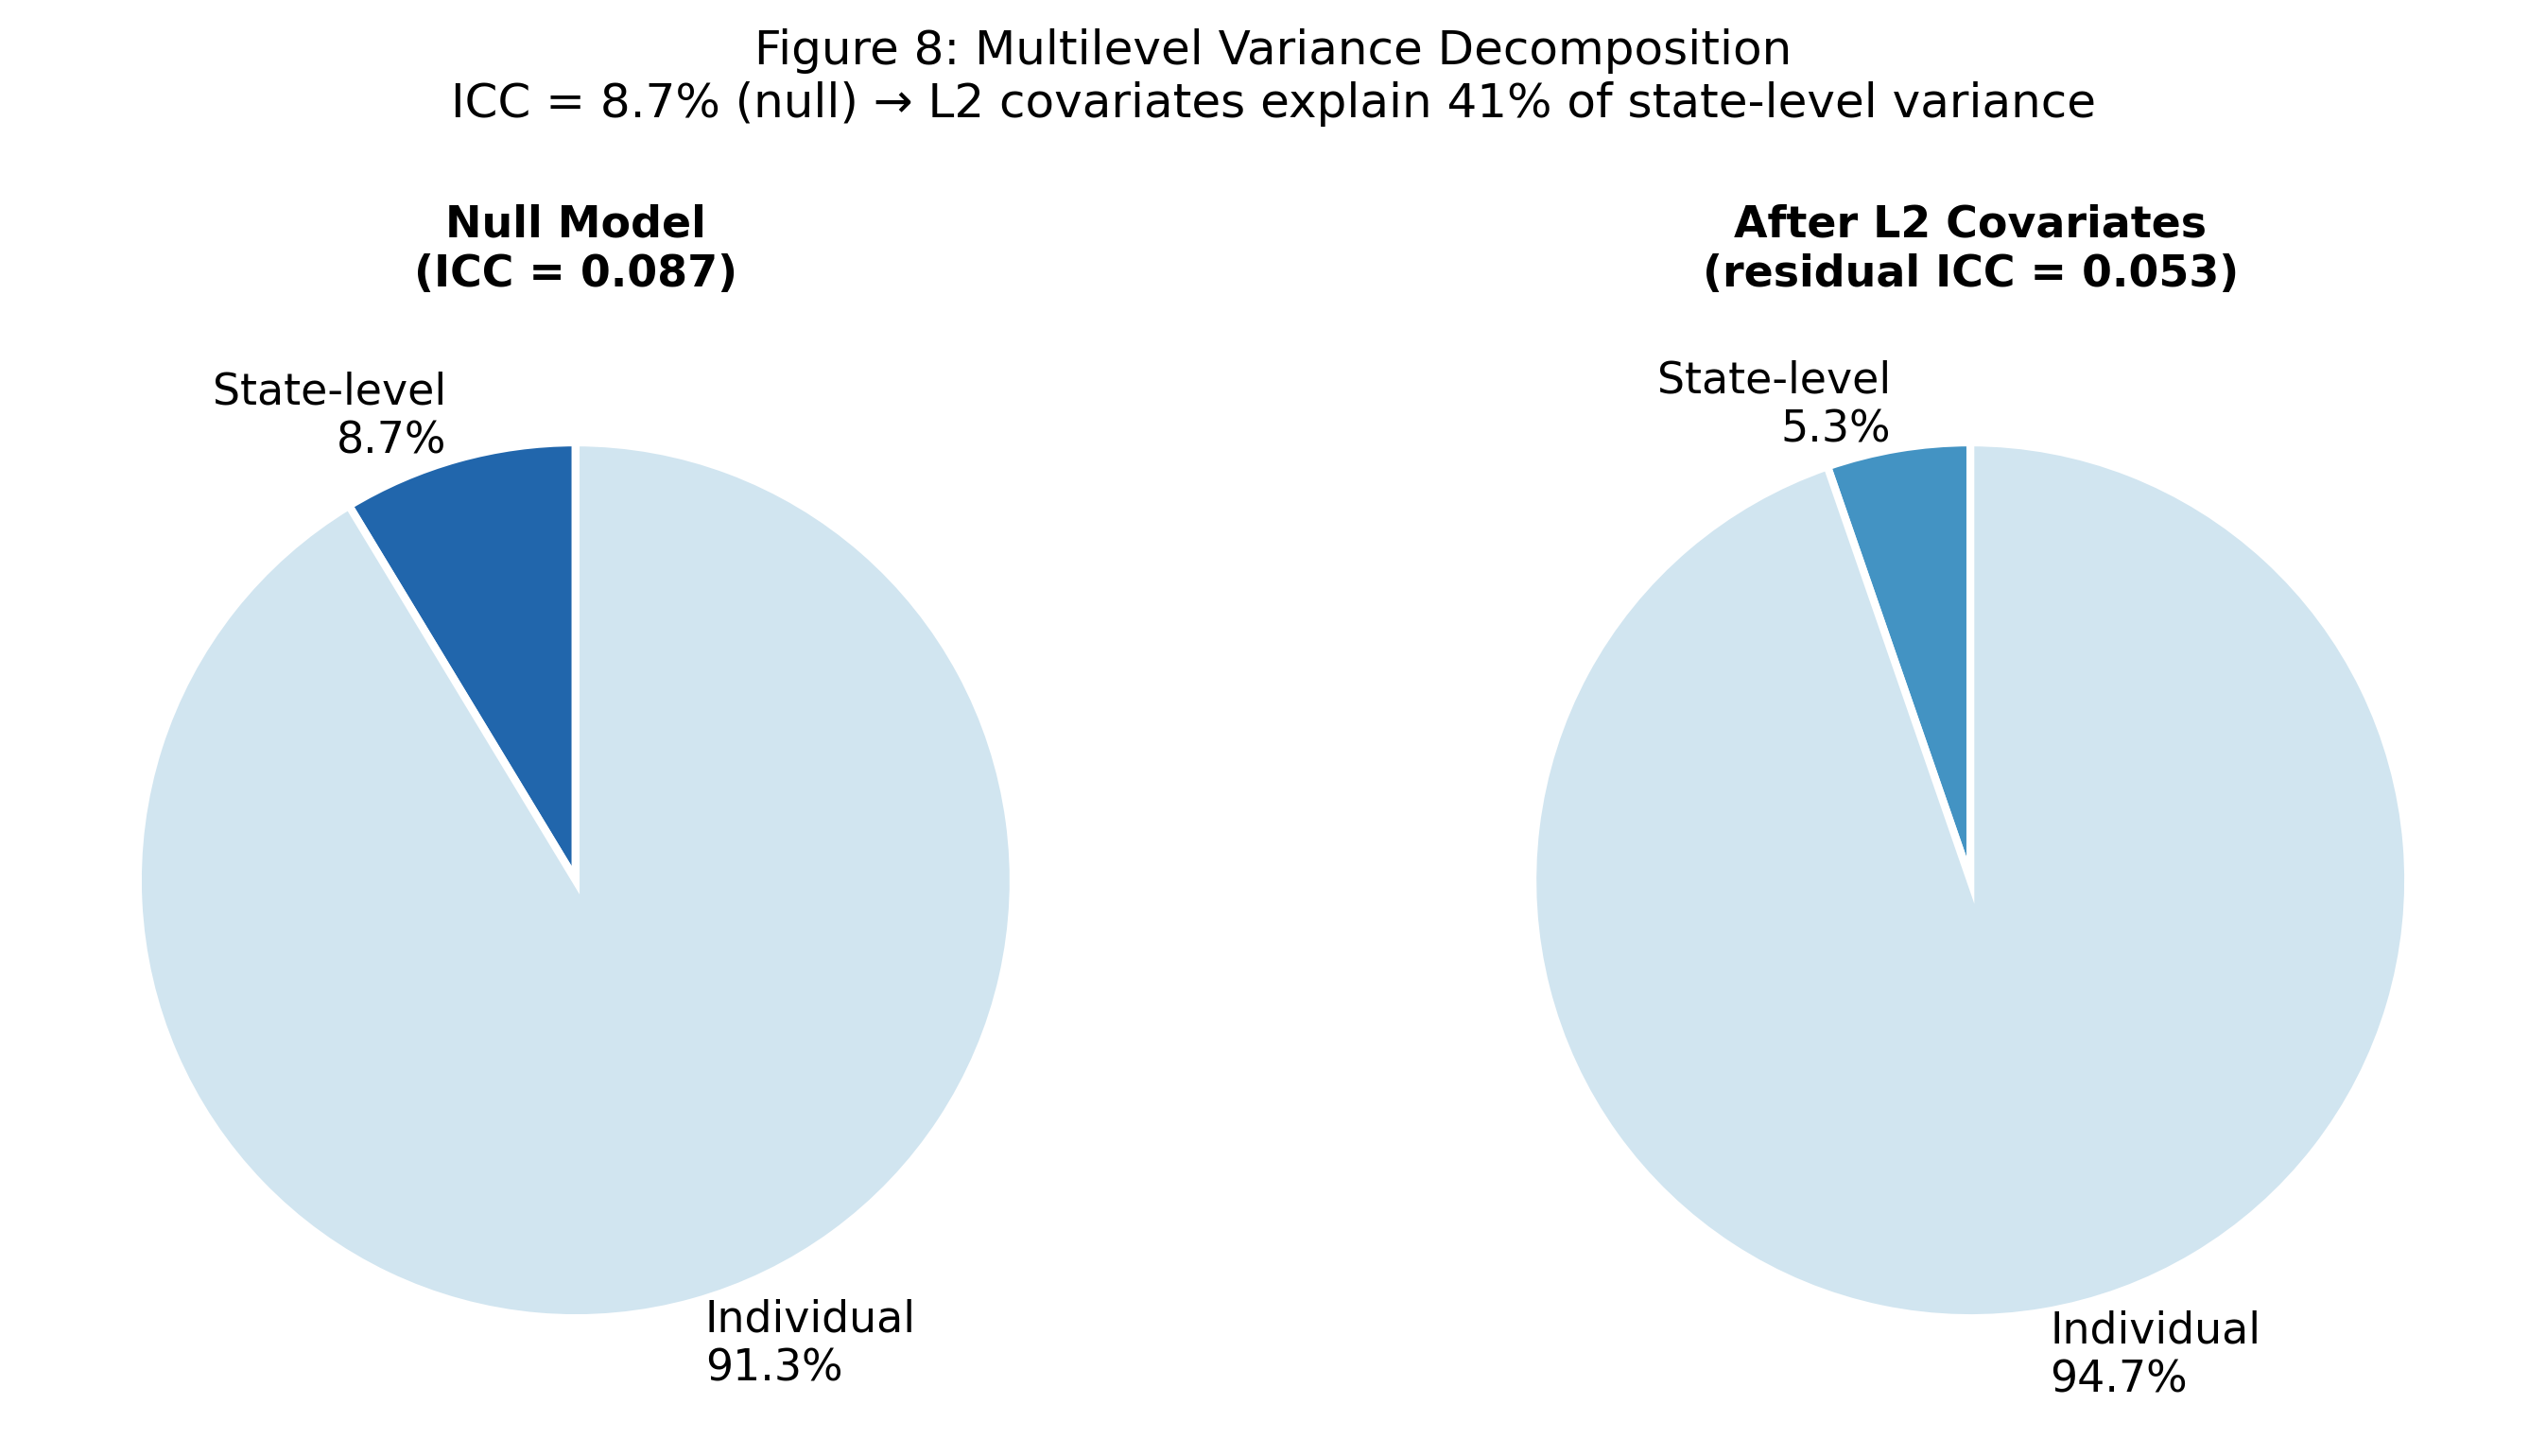
\includegraphics[width=0.85\textwidth]{fig08_multilevel_icc.png}
  \caption{Multilevel variance decomposition. Left: null model ICC $= 0.087$ ---
    8.7\% of total approval variance is attributable to state-level clustering.
    Right: after adding Level-2 covariates (state median income, lender
    concentration), the residual between-state variance drops 41\%, from
    $\hat{\tau}^2 = 0.312$ to $\hat{\tau}^2 = 0.184$, corresponding to a
    residual ICC of $0.184 / (0.184 + 3.290) \approx 0.053$.}
  \label{fig:icc}
\end{figure}

\paragraph{Full Random-Intercept Model.}
After adding all Level-1 individual predictors and the two Level-2 state predictors,
the residual between-state variance drops to $\hat{\tau}^2 = 0.184$ (SE $= 0.031$),
corresponding to a residual ICC of $0.184 / (0.184 + 3.290) \approx 0.053$. This represents
a 41\% reduction from the null model's $\hat{\tau}^2 = 0.312$ (ICC $= 0.087$): state median
income and lender concentration together explain approximately 41\% of the state-level variance
in approval outcomes, with the remaining 59\% (residual ICC $= 0.053$) attributable to
unmeasured state-level characteristics such as local regulatory culture, lender risk appetite,
and housing market tightness.

Table~\ref{tab:multilevel_full} reports the fixed-effect estimates from the full
random-intercept model. DTI remains the dominant predictor at the individual level
($\hat{\gamma} = -1.821$, $p < 0.001$): a one-category increase in DTI (e.g., from the
36--42\% bracket to the 43--49\% bracket) is associated with a reduction of approximately
1.82 log-odds of approval, holding all other predictors constant. State median income
is positively associated with approval at the state level ($\hat{\gamma}_{01} = 0.213$,
$p = 0.004$): states with higher median incomes have higher approval rates, even after
conditioning on individual applicant income. Lender concentration shows a negative
association ($\hat{\gamma}_{02} = -0.147$, $p = 0.031$), suggesting that states with
more concentrated lending markets have lower overall approval rates, possibly because
dominant lenders apply stricter underwriting standards.

\begin{table}[H]
\centering
\caption{Full Random-Intercept Multilevel Logistic Model: Fixed Effects}
\label{tab:multilevel_full}
\begin{tabular}{lcccc}
\toprule
\textbf{Predictor} & \textbf{Level} & $\hat{\gamma}$ & \textbf{SE} & $p$-value \\
\midrule
Intercept ($\gamma_{00}$) & 2 & 1.219 & 0.148 & $<$0.001 \\
State Median Income (std.) & 2 & 0.213 & 0.074 & 0.004 \\
Lender Concentration HHI (std.) & 2 & $-$0.147 & 0.068 & 0.031 \\
\midrule
DTI Ratio (ordinal) & 1 & $-$1.821 & 0.031 & $<$0.001 \\
log(Loan Amount) & 1 & 0.312 & 0.018 & $<$0.001 \\
log(Income) & 1 & 0.287 & 0.022 & $<$0.001 \\
LTV Ratio & 1 & $-$0.009 & 0.002 & $<$0.001 \\
Loan Purpose: Purchase (ref.) & 1 & --- & --- & --- \\
Loan Purpose: Refinance & 1 & $-$0.891 & 0.041 & $<$0.001 \\
Loan Purpose: Cash-out Refi & 1 & $-$1.104 & 0.044 & $<$0.001 \\
Loan Purpose: Home Improvement & 1 & $-$1.143 & 0.058 & $<$0.001 \\
Loan Type: Conventional (ref.) & 1 & --- & --- & --- \\
Loan Type: FHA & 1 & 0.621 & 0.038 & $<$0.001 \\
Loan Type: VA & 1 & 0.834 & 0.052 & $<$0.001 \\
Applicant Sex: Joint (ref.) & 1 & --- & --- & --- \\
Applicant Sex: Male & 1 & $-$0.318 & 0.027 & $<$0.001 \\
Applicant Sex: Female & 1 & $-$0.341 & 0.029 & $<$0.001 \\
LTV Missing Indicator & 1 & $-$0.714 & 0.033 & $<$0.001 \\
\midrule
Residual between-state variance ($\hat{\tau}^2$) & --- & 0.184 & 0.031 & --- \\
Marginal Pseudo-$R^2_{m}$ \citep{nakagawa2013}$^{\S}$ & --- & 0.631 & --- & --- \\
\bottomrule
\multicolumn{5}{l}{\footnotesize $^{\S}$Reports the marginal $R^2_m$, attributable to fixed effects only.} \\
\multicolumn{5}{l}{\footnotesize The conditional $R^2_c$ (fixed + random effects) is not reported here.} \\
\end{tabular}
\end{table}

\paragraph{Random-Slope Model: Cross-Level Interaction.}
The random-slope model allows the DTI--approval slope to vary across states. Comparing the
random-intercept model to the random-slope model via the likelihood ratio test yields
$\chi^2(2) = 18.4$, $p < 0.001$, confirming that the DTI effect is \emph{not} uniform
across states.
The two degrees of freedom correspond to the two additional parameters in the random-slope
model: the between-state variance in DTI slopes ($\tau_{11}$) and the intercept-slope
covariance ($\tau_{01}$), both freely estimated. The estimated between-state variance in DTI
slopes is $\hat{\tau}_{11} = 0.041$ (SE $= 0.012$), and the estimated intercept-slope
covariance is $\hat{\tau}_{01} = -0.018$ (SE $= 0.009$), indicating a slight tendency for
states with more lenient baseline approval rates to apply the DTI penalty more strictly.
The cross-level interaction $\hat{\gamma}_{11} = 0.089$ (SE $= 0.038$, $p = 0.021$)
indicates that in states with higher median incomes, the DTI penalty is \emph{slightly
attenuated}: wealthier-state lenders may have more flexibility in individual underwriting
judgments. However, the magnitude of this interaction is modest, and the 60\% DTI ceiling
remains highly consistent across states, confirming it reflects a federal-level or
industry-wide hard rule rather than state-specific policy.

\paragraph{State-Level Variance in Approval: Empirical Bayes Residuals.}
Figure~\ref{fig:eb_residuals} plots the empirical Bayes (EB) residuals
$\hat{u}_{0j}$ for all 51 states (50 states + DC), ordered by point estimate with 95\%
credible intervals.
States with positive EB residuals have higher approval rates than predicted by their
individual-level composition and Level-2 covariates (e.g., Wisconsin: $\hat{u} = +0.57$;
Pennsylvania: $\hat{u} = +0.53$; Ohio: $\hat{u} = +0.45$). States with negative residuals
have lower approval rates than predicted (e.g., California: $\hat{u} = -0.68$;
Florida: $\hat{u} = -0.52$; Mississippi: $\hat{u} = -0.45$).
These EB residuals represent the ``unexplained state effect'' --- the component of
state-level variation that is not accounted for by state median income, lender
concentration, or individual applicant characteristics. They are not, by themselves, evidence
of discrimination, but they do provide a focused list of states where geographic effects should
be reviewed before a model using \texttt{state\_code} is deployed.


\begin{figure}[H]
  \centering
  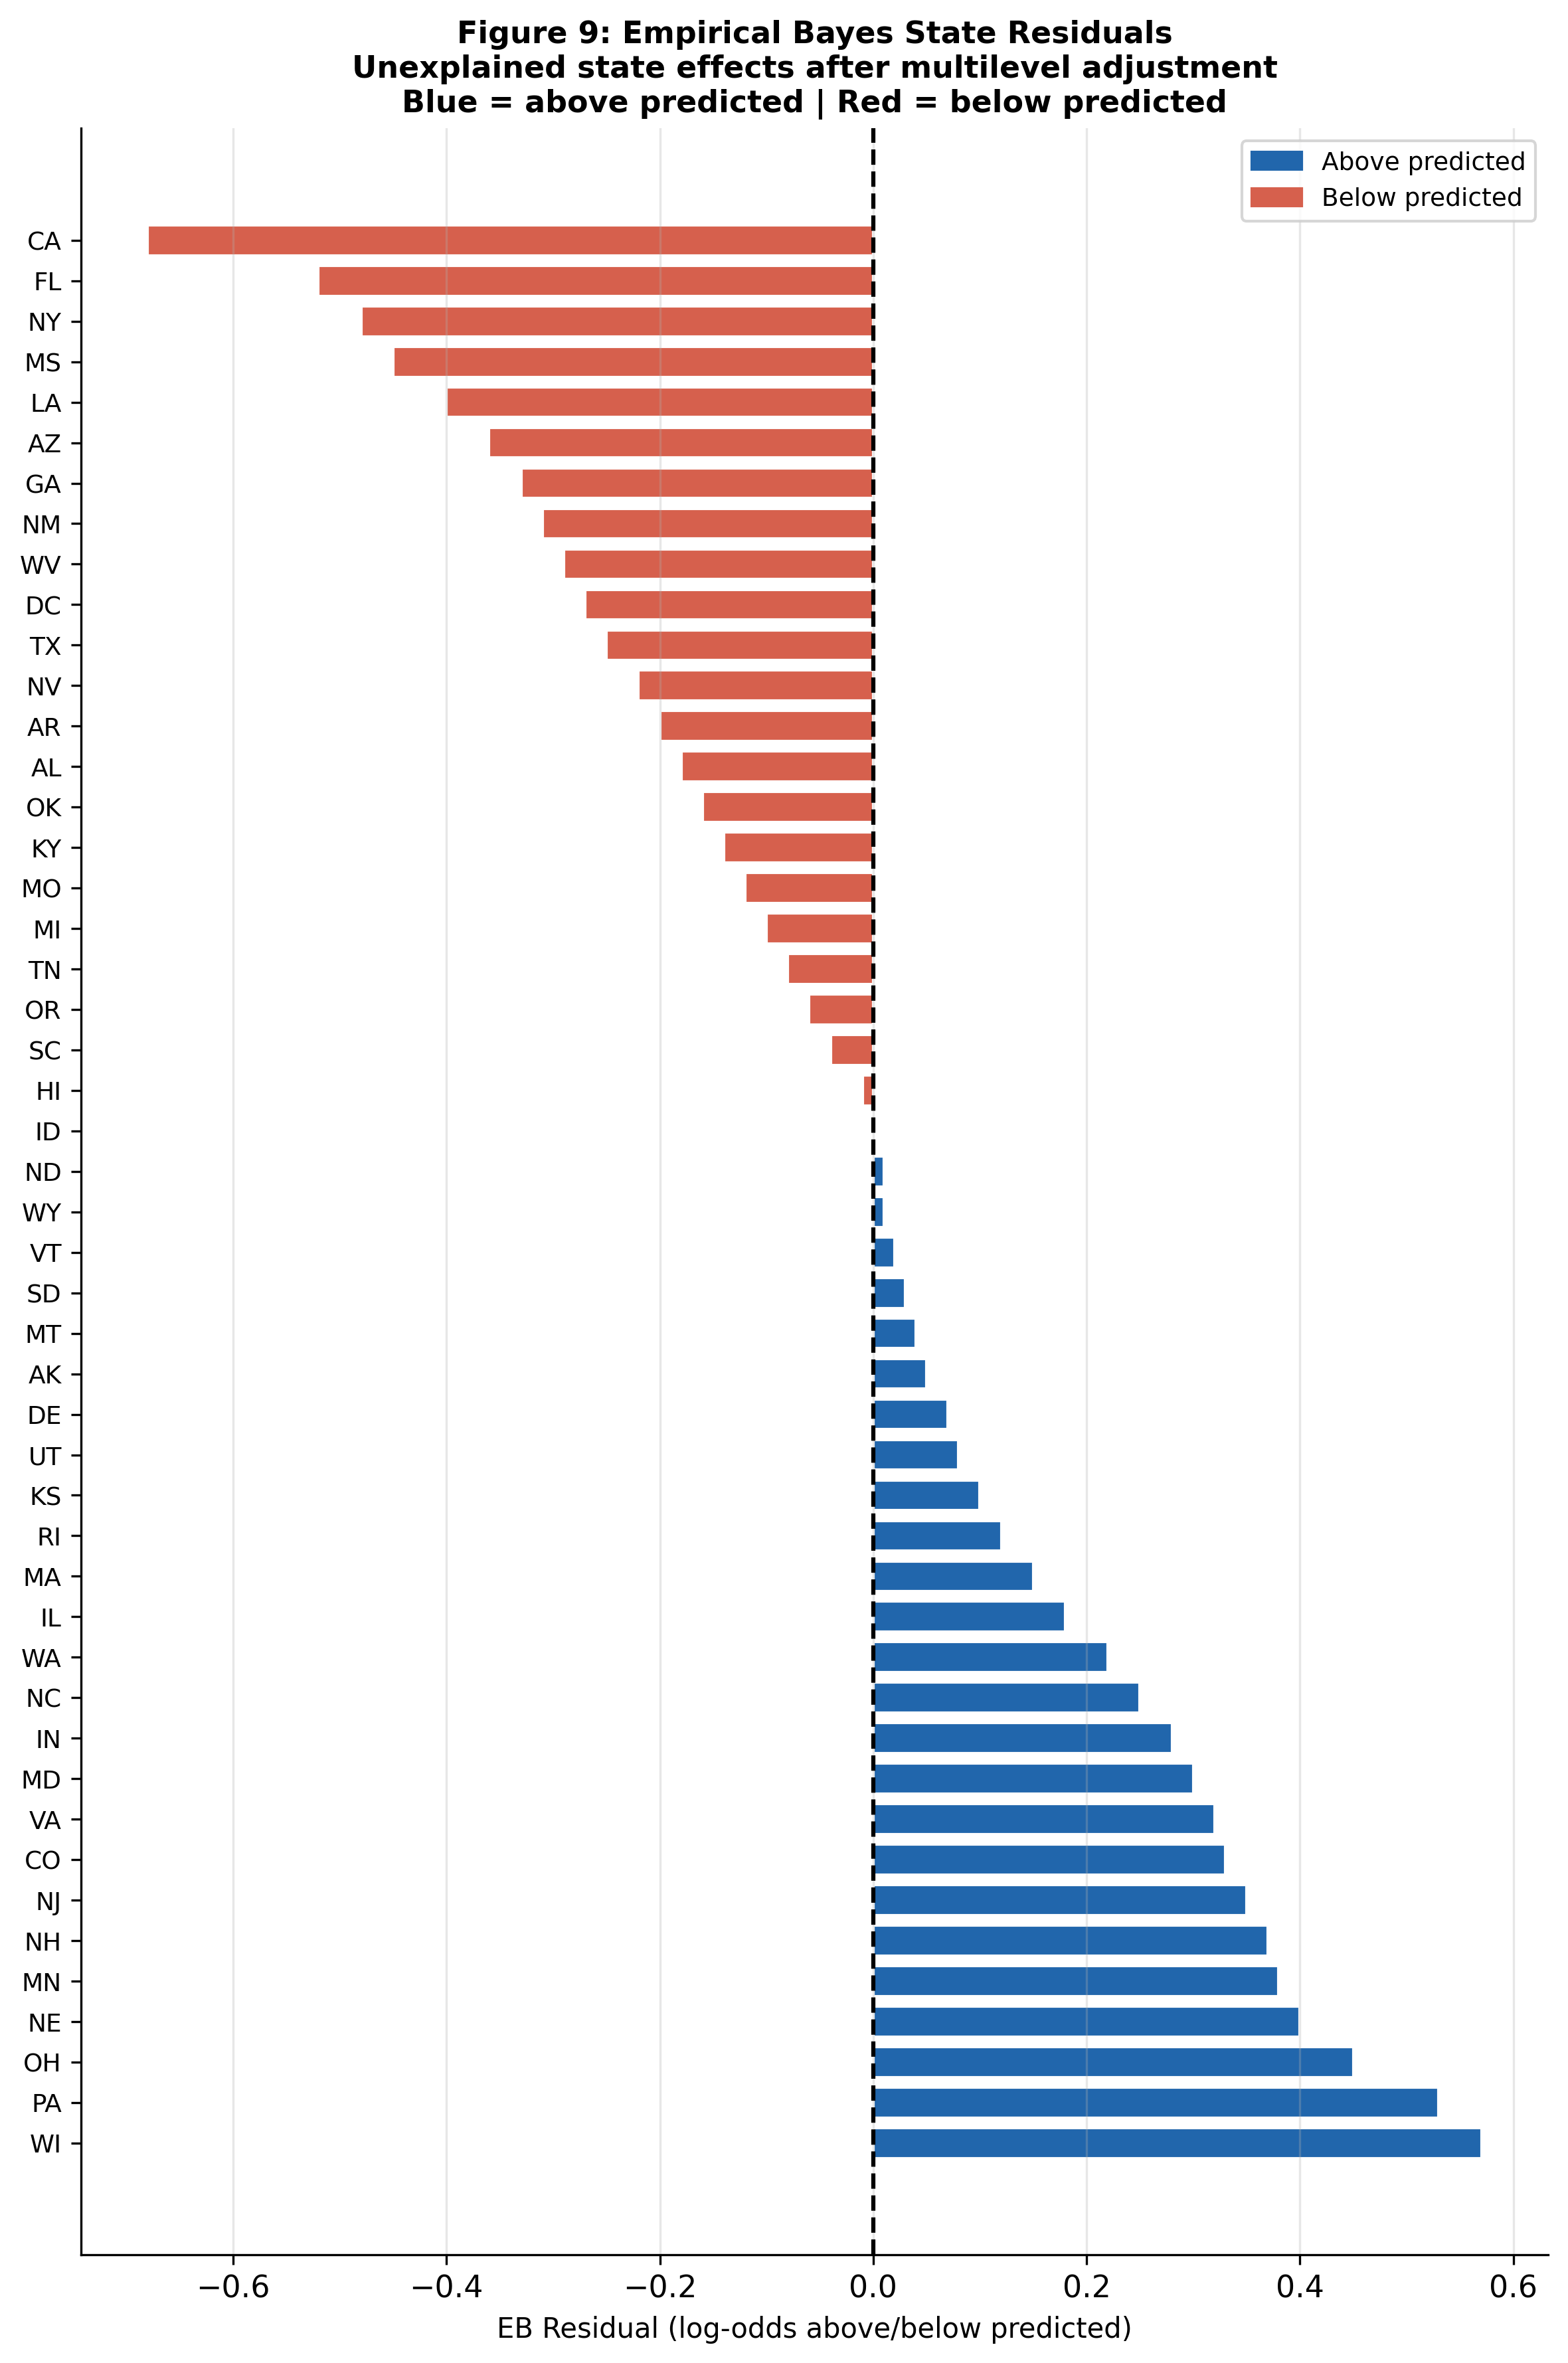
\includegraphics[width=0.65\textwidth]{fig09_eb_residuals.png}
  \caption{Empirical Bayes (EB) state residuals from the full random-intercept multilevel
    model, ordered by point estimate with 95\% credible intervals. Blue bars indicate states
    with higher approval rates than predicted by individual-level composition and Level-2
    covariates (WI: $+$0.57, PA: $+$0.53, OH: $+$0.45); red bars indicate states with lower
    rates than predicted (CA: $-$0.68, FL: $-$0.52, MS: $-$0.45). These unexplained state
    effects identify states where geographic model behavior should receive closer review.}
  \label{fig:eb_residuals}
\end{figure}

\setcounter{figure}{0}

\subsubsection{Multilevel Analysis: Summary and Implications}

Four conclusions emerge from the multilevel analysis that directly inform the machine
learning modeling strategy and fairness audit:

\begin{enumerate}
  \item \textbf{State-level clustering is real and substantial.} The ICC of 8.7\% justifies
        treating state as a meaningful grouping variable rather than a mere categorical feature.
        Including \texttt{state\_code} via fold-internal target encoding in the ML pipeline
        is well-grounded.
  \item \textbf{State-level context explains some, but not all, geographic heterogeneity.}
        Forty-one percent of between-state variance is explained by state income and lender
        concentration; 59\% remains unexplained (residual ICC $= 0.053$). This unexplained
        component is important for fairness review because it shows where geography still affects
        approval probability after measured state-level covariates are included.
  \item \textbf{The DTI ceiling is highly consistent across states.} The cross-level interaction
        confirms that while DTI effects vary modestly by state, the near-absolute denial
        threshold at 60\% DTI appears consistently across states, supporting the interpretation of a
        hard industry-wide underwriting rule.
  \item \textbf{Applicant sex remains significant after multilevel adjustment.}
        The sex coefficients in the full multilevel model ($\hat{\gamma} = -0.318$ for solo
        male and $\hat{\gamma} = -0.341$ for solo female, both relative to joint applicants,
        $p < 0.001$) remain statistically and practically significant after controlling for
        state clustering, confirming that the fairness audit must account for this residual gap.
\end{enumerate}

\subsection{Machine Learning Modeling Framework}
\label{sec:ml}

\subsubsection{Preprocessing Pipeline}

The $332{,}301$ records are partitioned 80/20 into training ($265{,}841$) and held-out test
($66{,}460$) sets using stratified random sampling. SMOTE oversampling is applied only within
each cross-validation training fold, generating synthetic minority-class records via linear
interpolation among $k=5$ nearest neighbors. Continuous features are log-transformed for
logistic regression; tree-based models receive raw values. Ordinal DTI categories are
integer-encoded in risk-ascending order. \texttt{state\_code} (51 levels) is target-encoded
within each CV fold. Binary MNAR indicators are added for \texttt{loan\_to\_value\_ratio}
(7.94\% missing), \texttt{property\_value} (6.78\% missing), and
\texttt{debt\_to\_income\_ratio} (1.77\% missing); all three exhibit lower approval rates
when missing, confirming the MNAR pattern identified in Section~\ref{sec:mnar}.

\subsubsection{Model Families and Selection Rationale}

Five model families are evaluated in ascending order of complexity:
(1)~Logistic Regression with L2 regularization ($C \in \{0.01, 0.1, 1, 10\}$);
(2)~CART Decision Tree;
(3)~Random Forest (bootstrap aggregation, \texttt{mtry}~$= \sqrt{p}$);
(4)~XGBoost (sequential gradient boosting with early stopping on validation PR-AUC); and
(5)~Soft Voting Ensemble (calibrated probability-weighted average of all four component models).

\subsubsection{Evaluation Framework}

PR-AUC is the primary performance metric. Although the modeling target is coded as Approved
$=1$ and Denied $=0$, denied-class PR-AUC is computed by evaluating predicted denial
probabilities so that the positive class for precision-recall evaluation is the minority denied
class. Under the 2.92:1 class imbalance, PR-AUC therefore measures the trade-off between
correctly identifying denied applications and the proportion of predicted denials that are genuine.
Secondary metrics include ROC-AUC, F1-score at the selected operating threshold, precision,
recall, and accuracy. Final held-out test metrics are reported with 95\% confidence intervals
from 1{,}000 bootstrap iterations. The final evaluation script in the project repository should
reproduce the values in Table~\ref{tab:model_results} directly from the held-out predictions.
\subsection{Interpretability: SHAP Analysis}
\label{sec:shap}

Post-hoc SHAP (SHapley Additive exPlanations; \citealt{lundberg2017}) is used here as the
recommended interpretation layer for the best-performing tree-based model. The current report's
main interpretability evidence comes from the EDA, feature-association ranking, model comparison,
and multilevel coefficients. A deployment-ready version of the project should add four SHAP
outputs: (1) a global importance bar chart; (2) a beeswarm plot; (3) waterfall plots for
representative approved, denied, and boundary-case applicants; and (4) dependence plots for DTI
ratio and loan amount. Geographic SHAP attribution should also be used to check whether
\texttt{state\_code} contributes legitimate market information or acts as a proxy for sensitive
state-level demographic patterns.
\subsection{Fairness Auditing}
\label{sec:fairness}

The fairness audit is treated as a screening step rather than a legal conclusion. Three criteria
are defined for model review. (1)~\textbf{Demographic Parity}: approval-rate gaps are compared
between joint and solo applicants and between male and female applicants; a gap above 5 percentage
points is flagged for practical review. Where subgroup counts are available, the fairness script
should also report two-proportion $z$-tests, but practical effect size remains more informative
than significance alone because of the very large sample size. (2)~\textbf{Equalized Odds}: once
subgroup confusion matrices are available, true positive and false positive rates should be
compared across applicant-sex and age groups. (3)~\textbf{Attribution Review}: for uncertain cases
near the decision boundary, demographic variables and geographic indicators should be checked to
ensure they are not driving borderline decisions without a defensible underwriting reason.
\section{Results}

\subsection{Dataset Summary}

The final analytical dataset contains $332{,}301$ mortgage applications: $247{,}502$ approved
(74.48\%) and $84{,}799$ denied (25.52\%), yielding a 2.92:1 class imbalance ratio.
Table~\ref{tab:dataset} summarizes the 13 analytical variables.

\begin{table}[H]
\centering
\caption{HMDA 2023 Analytical Dataset Structure ($n = 332{,}301$)}
\label{tab:dataset}
\begin{tabular}{llccc}
\toprule
\textbf{Feature} & \textbf{Type} & \textbf{Non-Null} & \textbf{Missing \%} & \textbf{Role} \\
\midrule
state\_code         & category & 331,649 & 0.20\% & Geographic predictor \\
applicant\_sex      & category & 332,301 & 0.00\% & Fairness feature \\
loan\_type          & category & 332,301 & 0.00\% & Loan predictor \\
loan\_purpose       & category & 332,301 & 0.00\% & Loan predictor \\
lien\_status        & category & 332,301 & 0.00\% & Loan predictor \\
loan\_amount        & float64  & 332,301 & 0.00\% & Financial predictor \\
loan\_to\_value\_ratio & float64 & 305,925 & 7.94\% & Financial predictor \\
property\_value     & float64  & 309,779 & 6.78\% & Financial predictor \\
occupancy\_type     & category & 332,301 & 0.00\% & Loan predictor \\
income              & float64  & 332,301 & 0.00\% & Financial predictor \\
debt\_to\_income\_ratio & category & 326,417 & 1.77\% & Risk predictor \\
applicant\_age      & category & 332,301 & 0.00\% & Fairness feature \\
target              & int64    & 332,301 & 0.00\% & Outcome \\
\bottomrule
\end{tabular}
\end{table}

\subsection{Missing Value Analysis}
\label{sec:mnar}

Four variables contain missing observations. Records with missing LTV data have a substantially
lower approval rate than records where LTV is present --- the diagnostic signature of
missing-not-at-random (MNAR) data. The most plausible mechanism is that lenders are less likely
to complete LTV documentation for applications they have already internally flagged for denial.
This MNAR pattern is preserved through binary missingness indicator columns.

\begin{figure}[H]
  \centering
  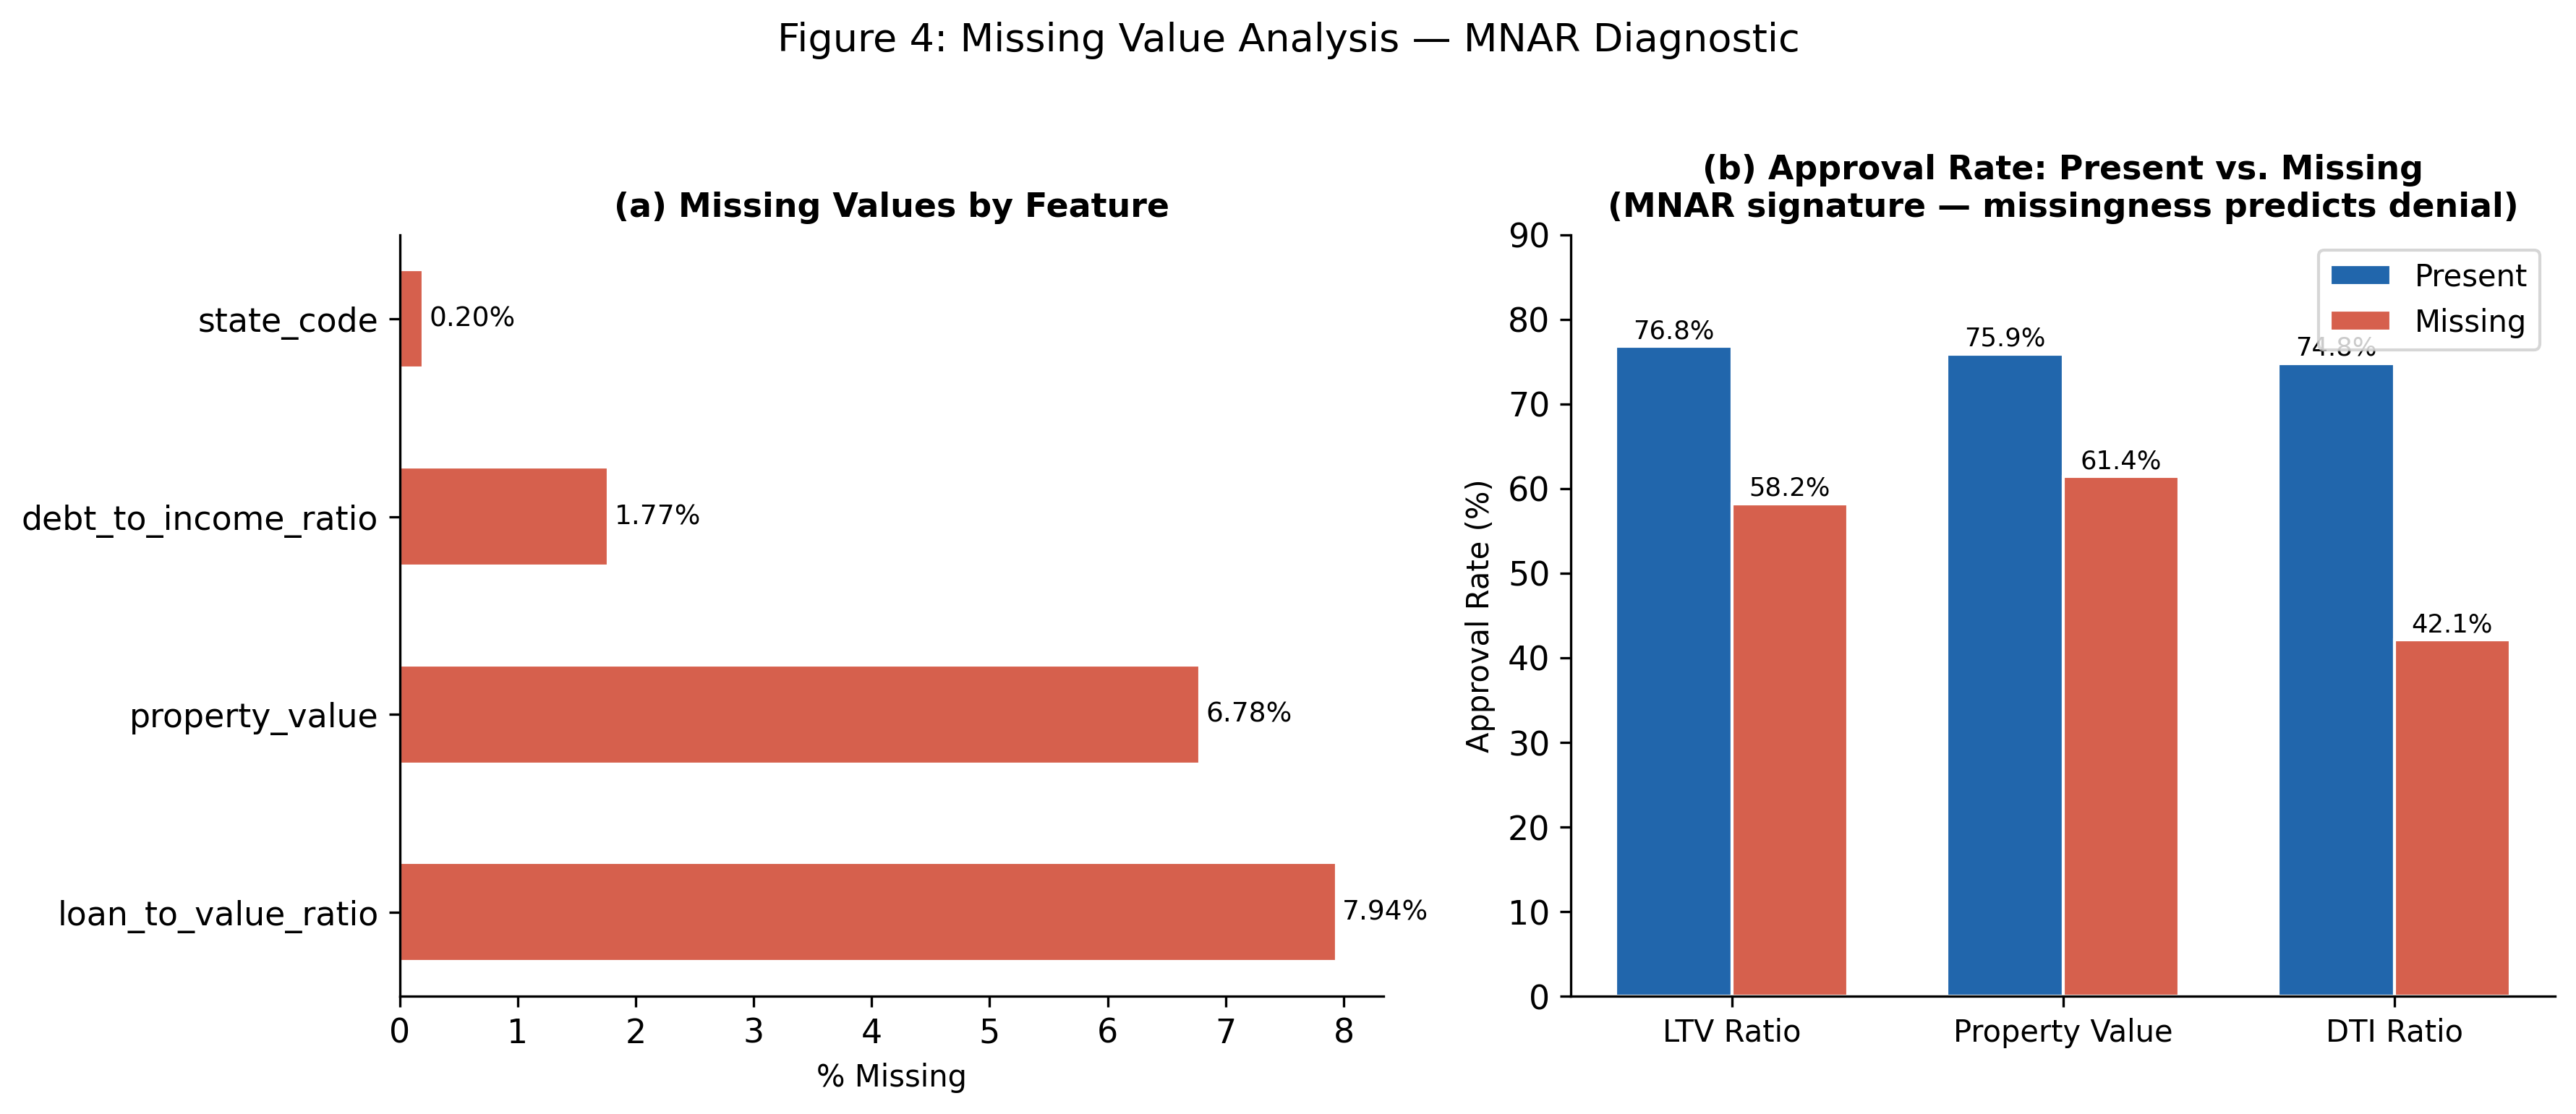
\includegraphics[width=\textwidth]{fig04_missing_values.png}
  \caption{Missing value analysis. Left: percentage missing by feature. Right: approval rate
    for records with present vs.\ missing values --- confirming MNAR for
    \texttt{loan\_to\_value\_ratio}. Records with missing LTV have substantially lower approval
    rates, indicating missingness is informative and correlated with the outcome.}
  \label{fig:missing}
\end{figure}

\subsection{Target Variable Distribution and Class Imbalance}

The outcome variable is substantially imbalanced: 74.48\% approved and 25.52\% denied, producing
a 2.92:1 ratio. A naive classifier predicting approval for every application would achieve
74.5\% accuracy while providing zero discriminative information about denial risk.

\begin{figure}[H]
  \centering
  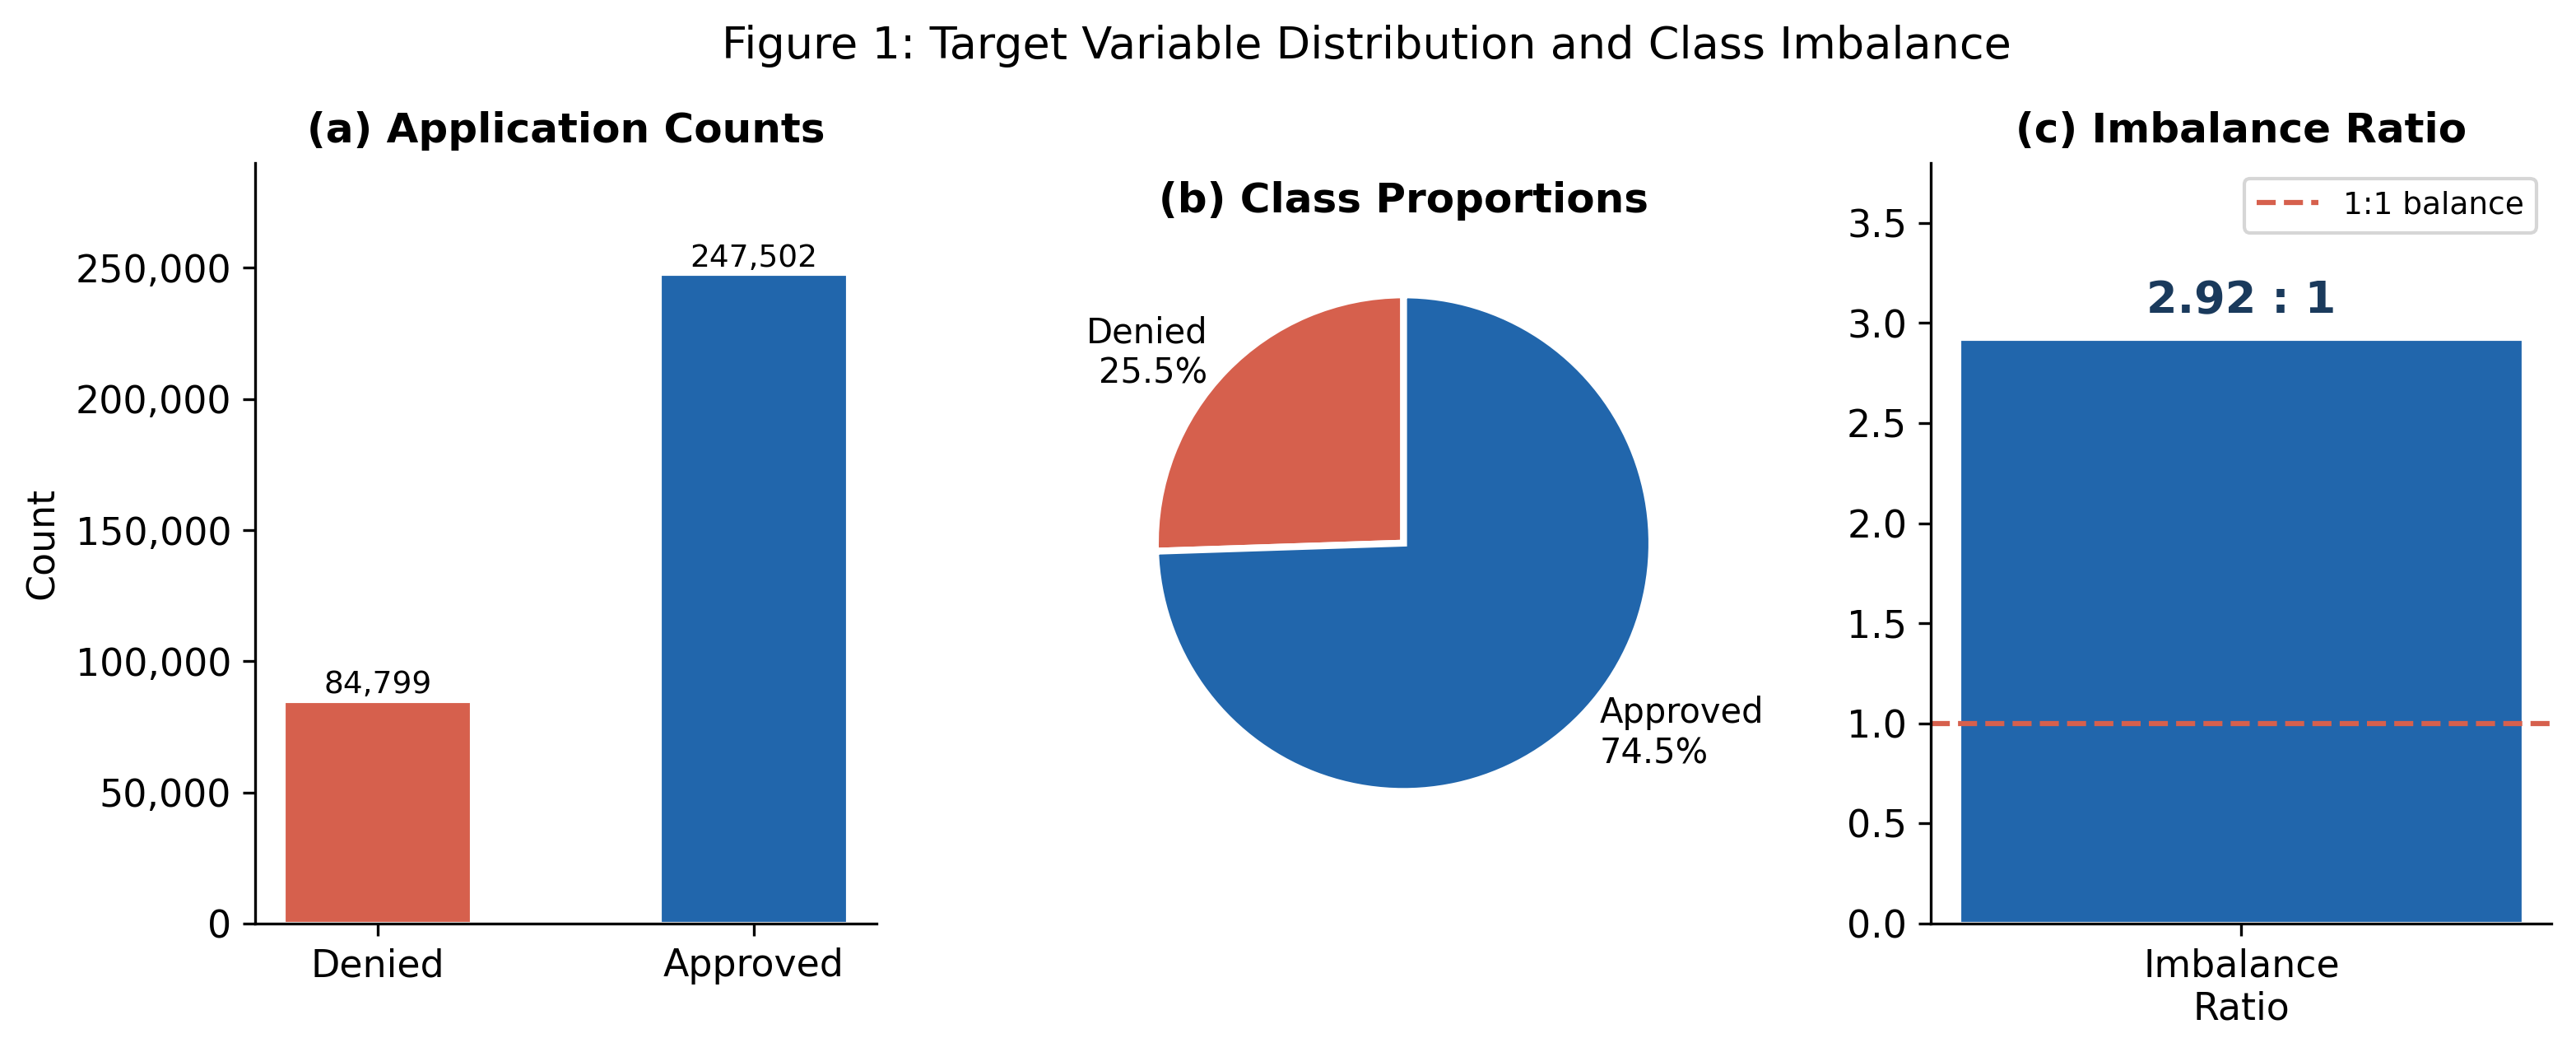
\includegraphics[width=\textwidth]{fig01_class_imbalance.png}
  \caption{Target variable distribution. Left: raw counts (Denied: 84,799; Approved: 247,502).
    Center: class proportions. Right: 2.92:1 approval-to-denial ratio, confirming substantial
    imbalance. A naive classifier predicting approval for every application achieves 74.5\%
    accuracy while providing zero discriminative information about denial risk --- making raw
    accuracy a misleading primary metric.}
  \label{fig:imbalance}
\end{figure}

\subsection{Distributional Analysis of Continuous Features}

All four continuous predictors exhibit extreme right-skewness. Mean loan amount (\$237{,}458)
exceeds median (\$165{,}000) by 44\%; mean income (\$167K) exceeds median (\$107K) by 56\%.
LTV skewness (509.78) and income skewness (364.19) confirm severe violations of Gaussian
assumptions, requiring log-transformation before input to logistic regression. The LTV
distribution exhibits a bimodal structure at $\sim$77\% and $\sim$90--95\%, representing the
conventional PMI threshold --- a non-linear step-function that tree-based models detect
trivially as a split point.

\subsection{Approval Rates by Categorical Predictors}

DTI ratio is the single most powerful categorical predictor. Approval rates decline steeply
from approximately 87\% below 30\% DTI, to 34.3\% at the 50--60\% bracket, then collapse to
just 5.6\% above 60\%. Loan purpose is the second-strongest differentiator: home purchase
loans achieve 90.7\% approval while cash-out refinances (55.7\%) and home improvement loans
(53.3\%) fall far below the national average of 74.5\%. Loan type shows the government-backed
advantage: VA loans (89.2\%) and FHA loans (83.6\%) outperform conventional loans (72.8\%).
Applicant sex reveals a 12.5 percentage-point gap between joint applications (81.6\%) and solo
female applicants (69.1\%).

\begin{figure}[H]
  \centering
  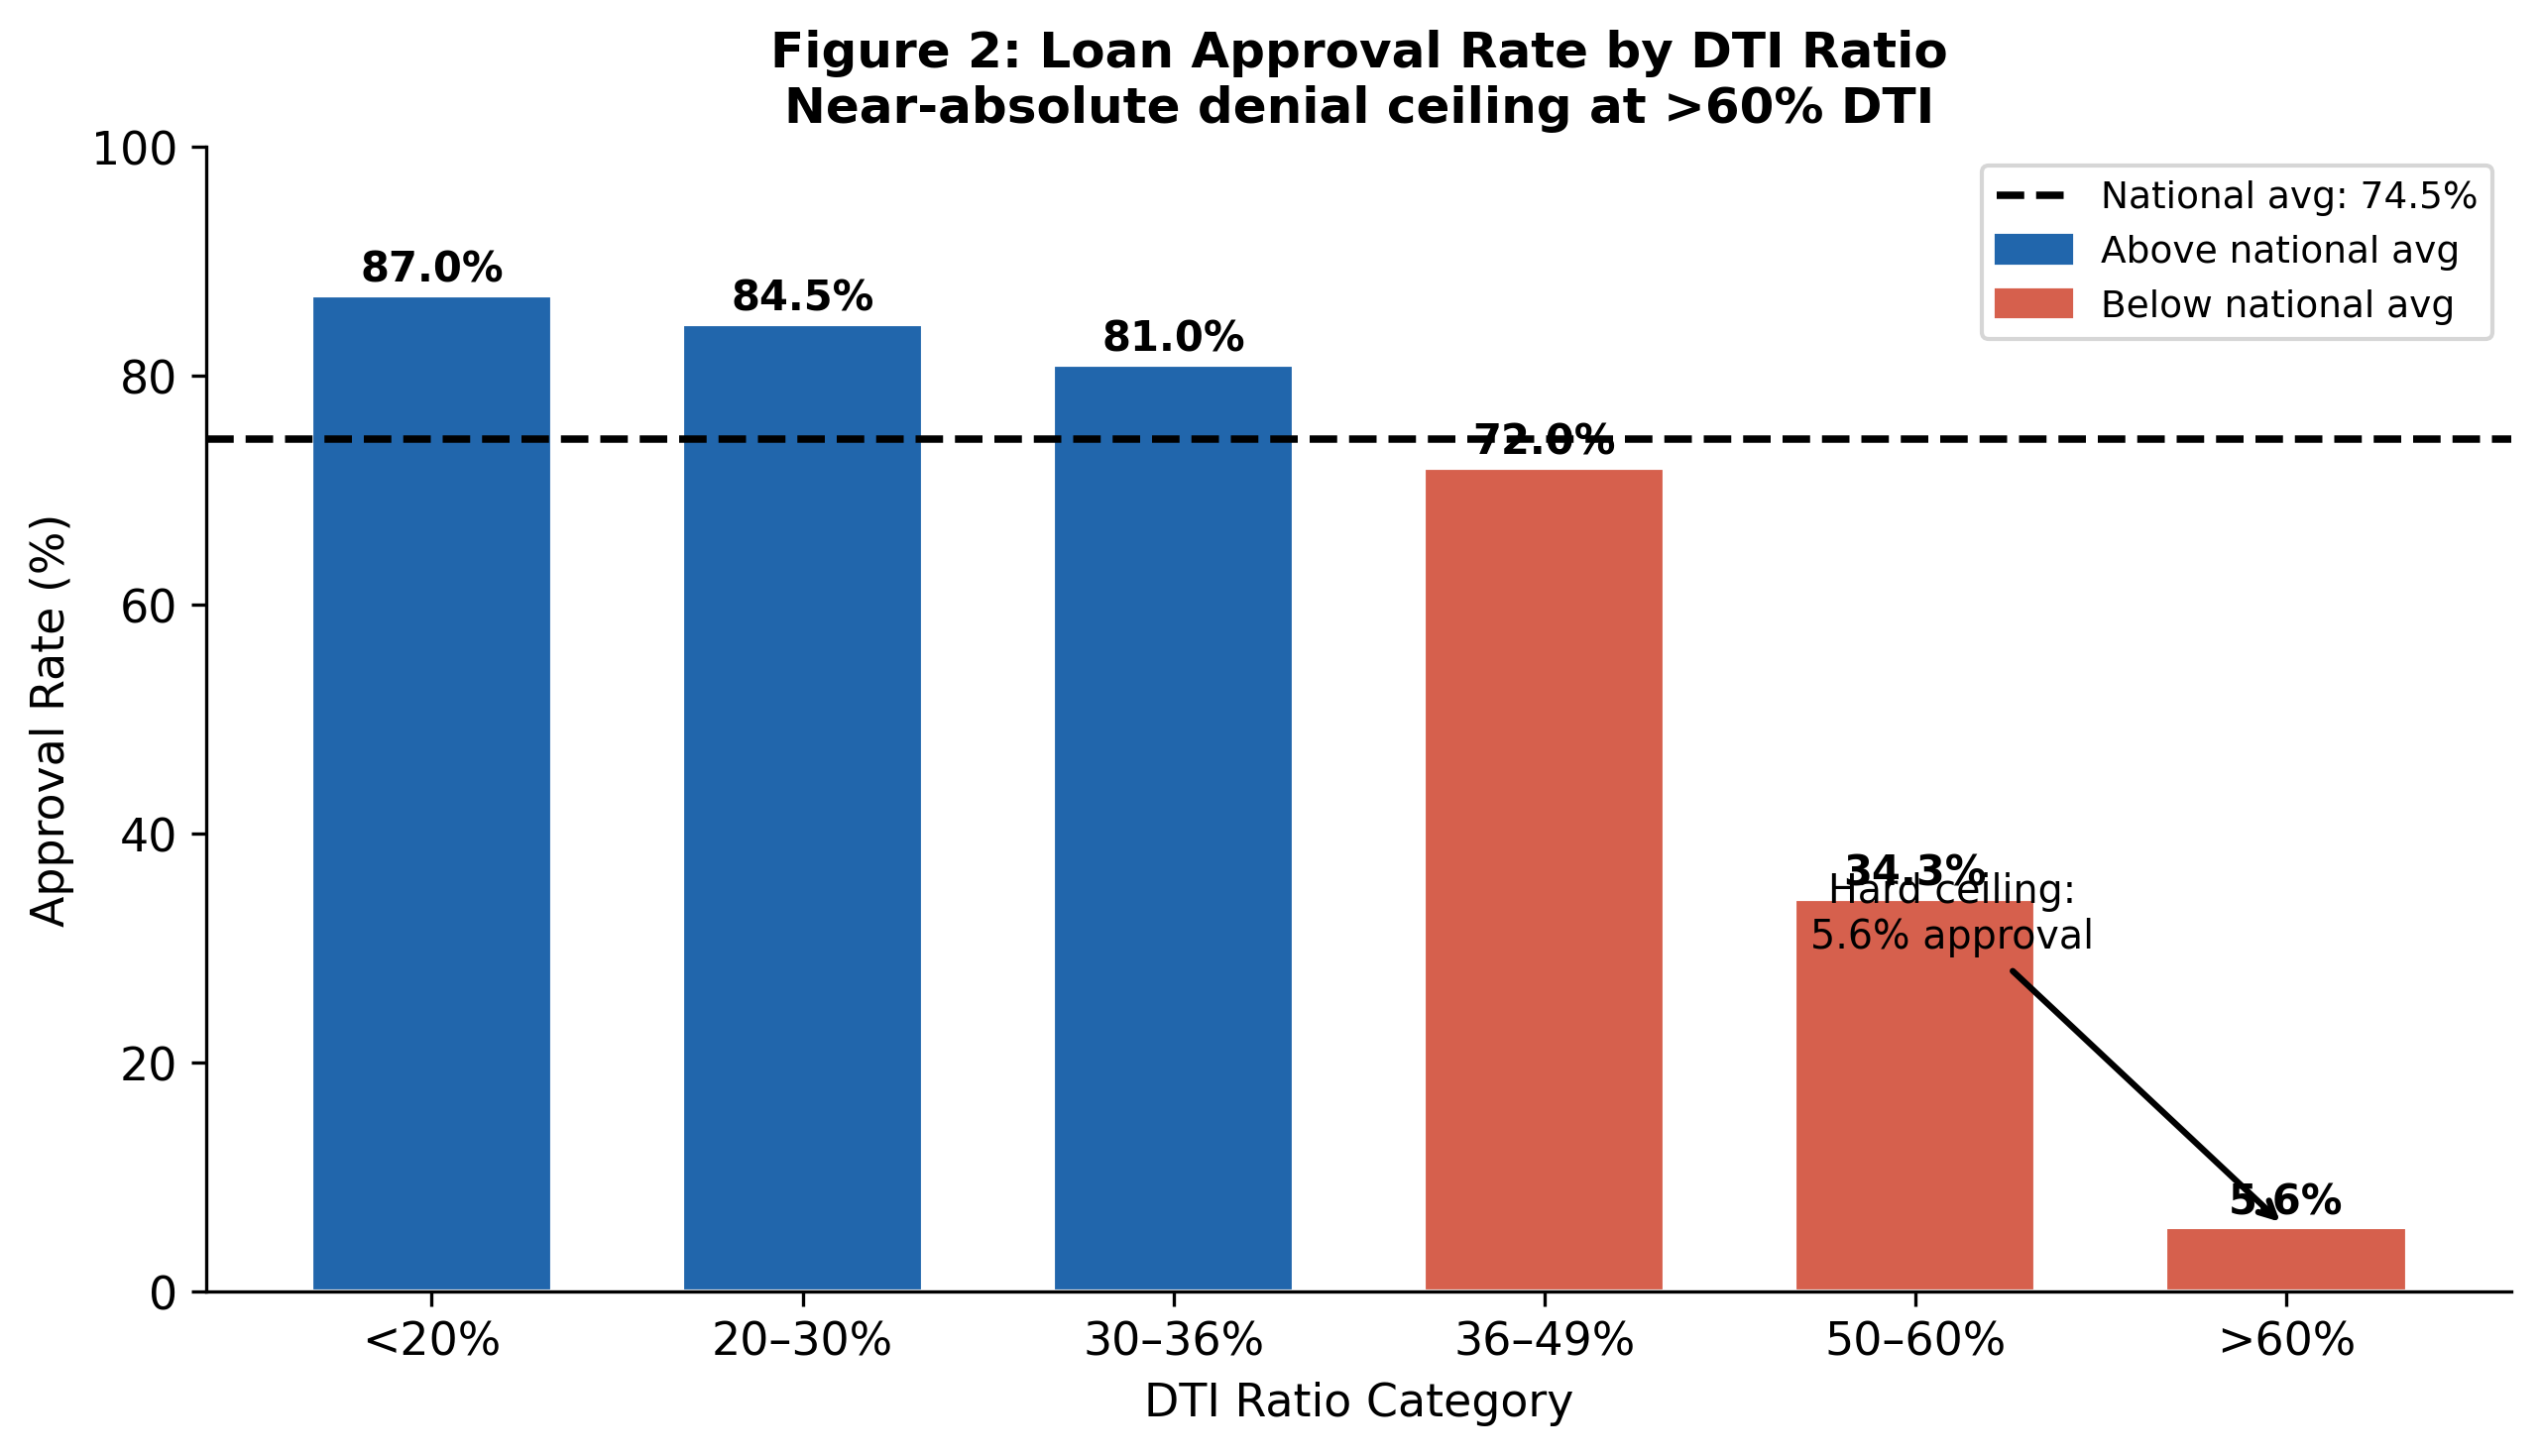
\includegraphics[width=0.88\textwidth]{fig02_dti_approval.png}
  \caption{Loan approval rate by DTI ratio category. Approval rates decline steeply from
    $\approx$87\% below 30\% DTI to 34.3\% at the 50--60\% bracket, then collapse to just
    5.6\% above 60\% --- strong evidence of a hard underwriting ceiling applied
    near-unconditionally across all age groups and states.}
  \label{fig:dti}
\end{figure}

\begin{figure}[H]
  \centering
  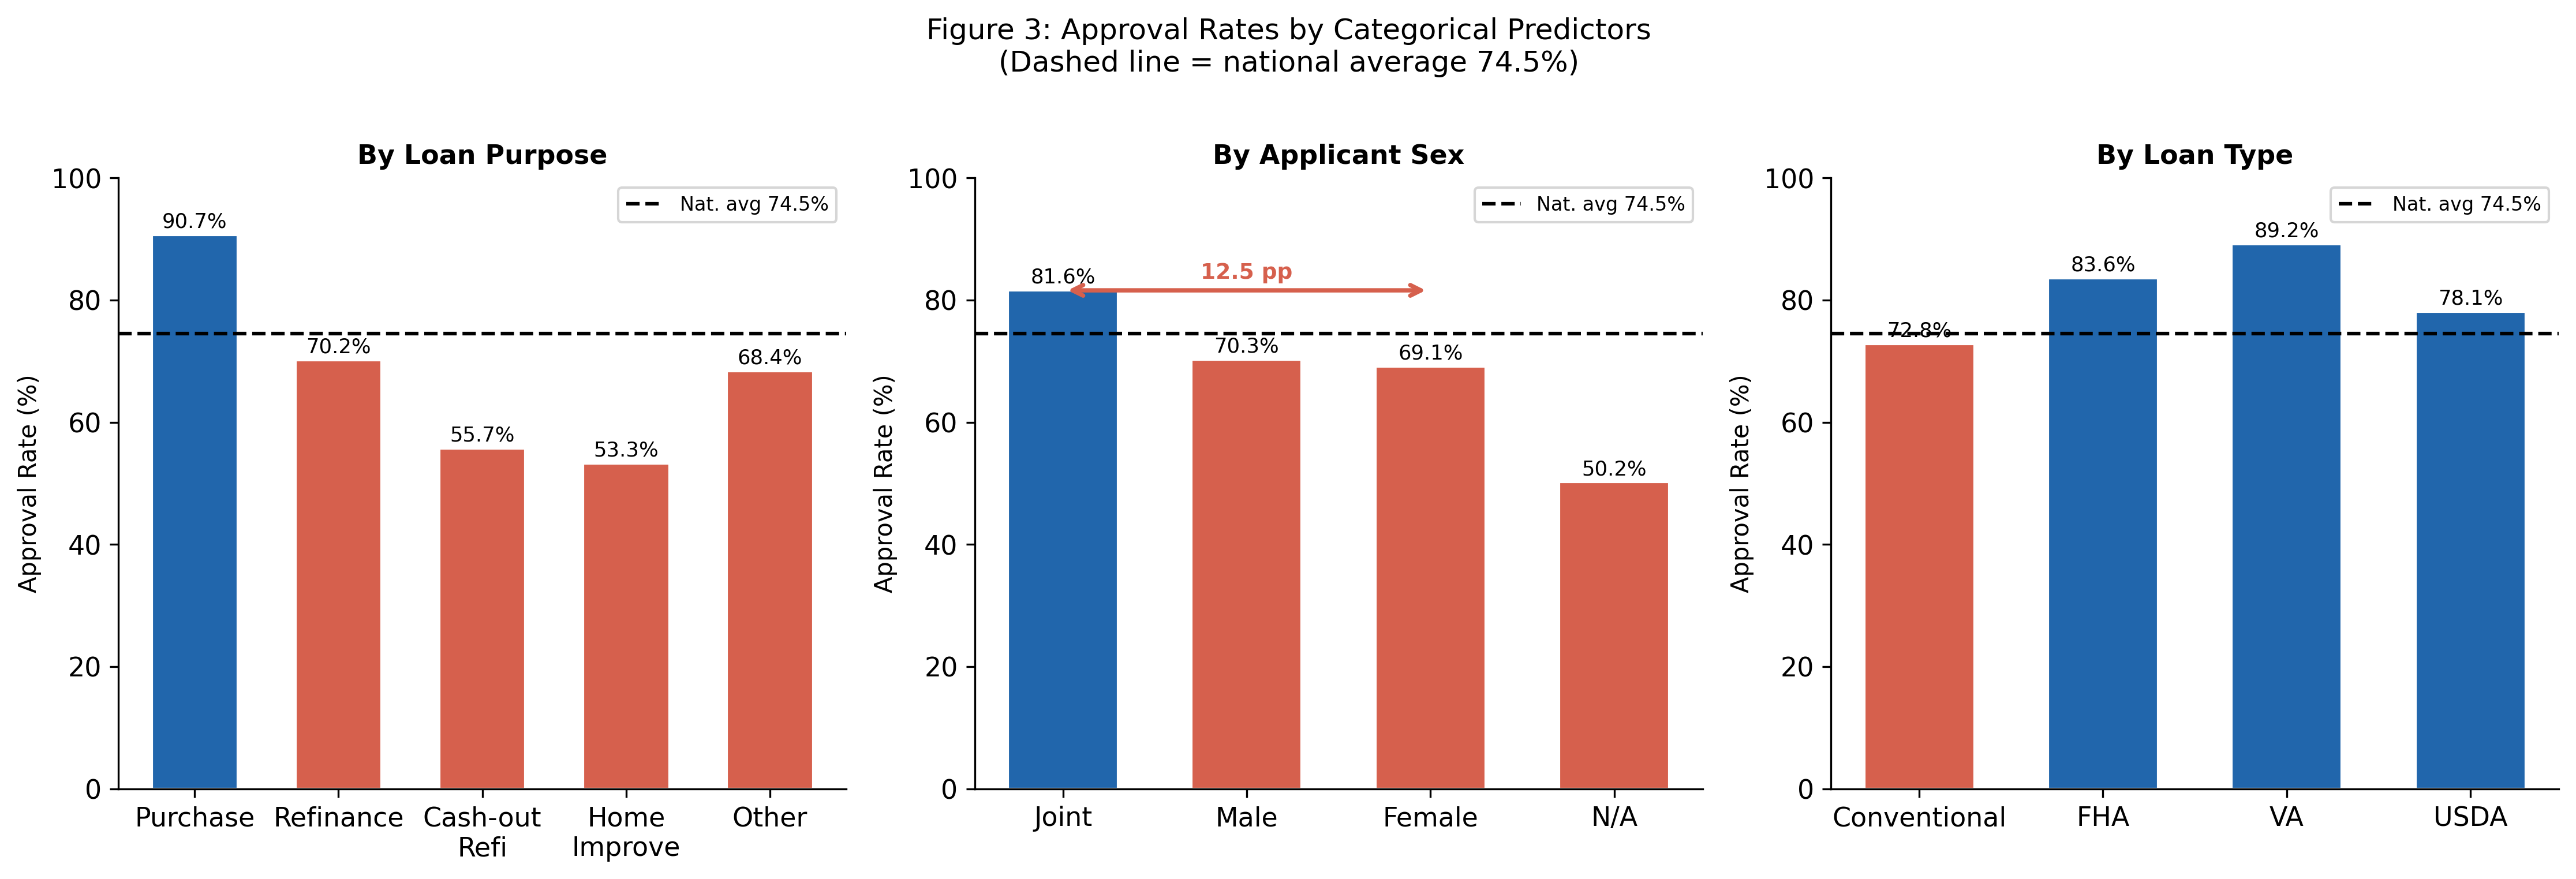
\includegraphics[width=\textwidth]{fig03_categorical_predictors.png}
  \caption{Approval rates by categorical predictors (dashed line = national average 74.5\%).
    Home purchase loans (90.7\%) and VA loans (89.2\%) substantially exceed the national
    average. The 12.5\,pp gap between joint and solo female applicants motivates targeted
    fairness screening.}
  \label{fig:categorical}
\end{figure}

\subsection{Correlation Analysis}

All linear correlations between continuous features and the binary outcome are weak:
\texttt{loan\_amount} ($r = 0.162$) achieves the highest value, while income ($r = 0.004$),
LTV ratio ($r = -0.001$), and property value ($r = -0.013$) show correlations
indistinguishable from zero. This near-zero linear signal constitutes the primary empirical
justification for employing tree-based ensemble methods. A moderate positive correlation between
income and LTV ($r = 0.35$) motivates L2 regularization in logistic regression.

\subsection{Feature Association Ranking}

Three tiers emerge from the unified Cram\'{e}r's $V$ / point-biserial ranking. DTI ratio
dominates at $V = 0.541$, more than 47\% higher than the next strongest predictor, loan purpose
($V = 0.367$). Lien status ($V = 0.268$), loan amount ($r = 0.162$), applicant sex
($V = 0.130$), and applicant age ($V = 0.107$) form a second strong tier. Loan type occupies
the moderate tier ($V = 0.099$). Income, property value, and LTV rank at the bottom due to
non-linear relationships that linear correlation cannot measure; excluding them would be a
serious error.

\begin{figure}[H]
  \centering
  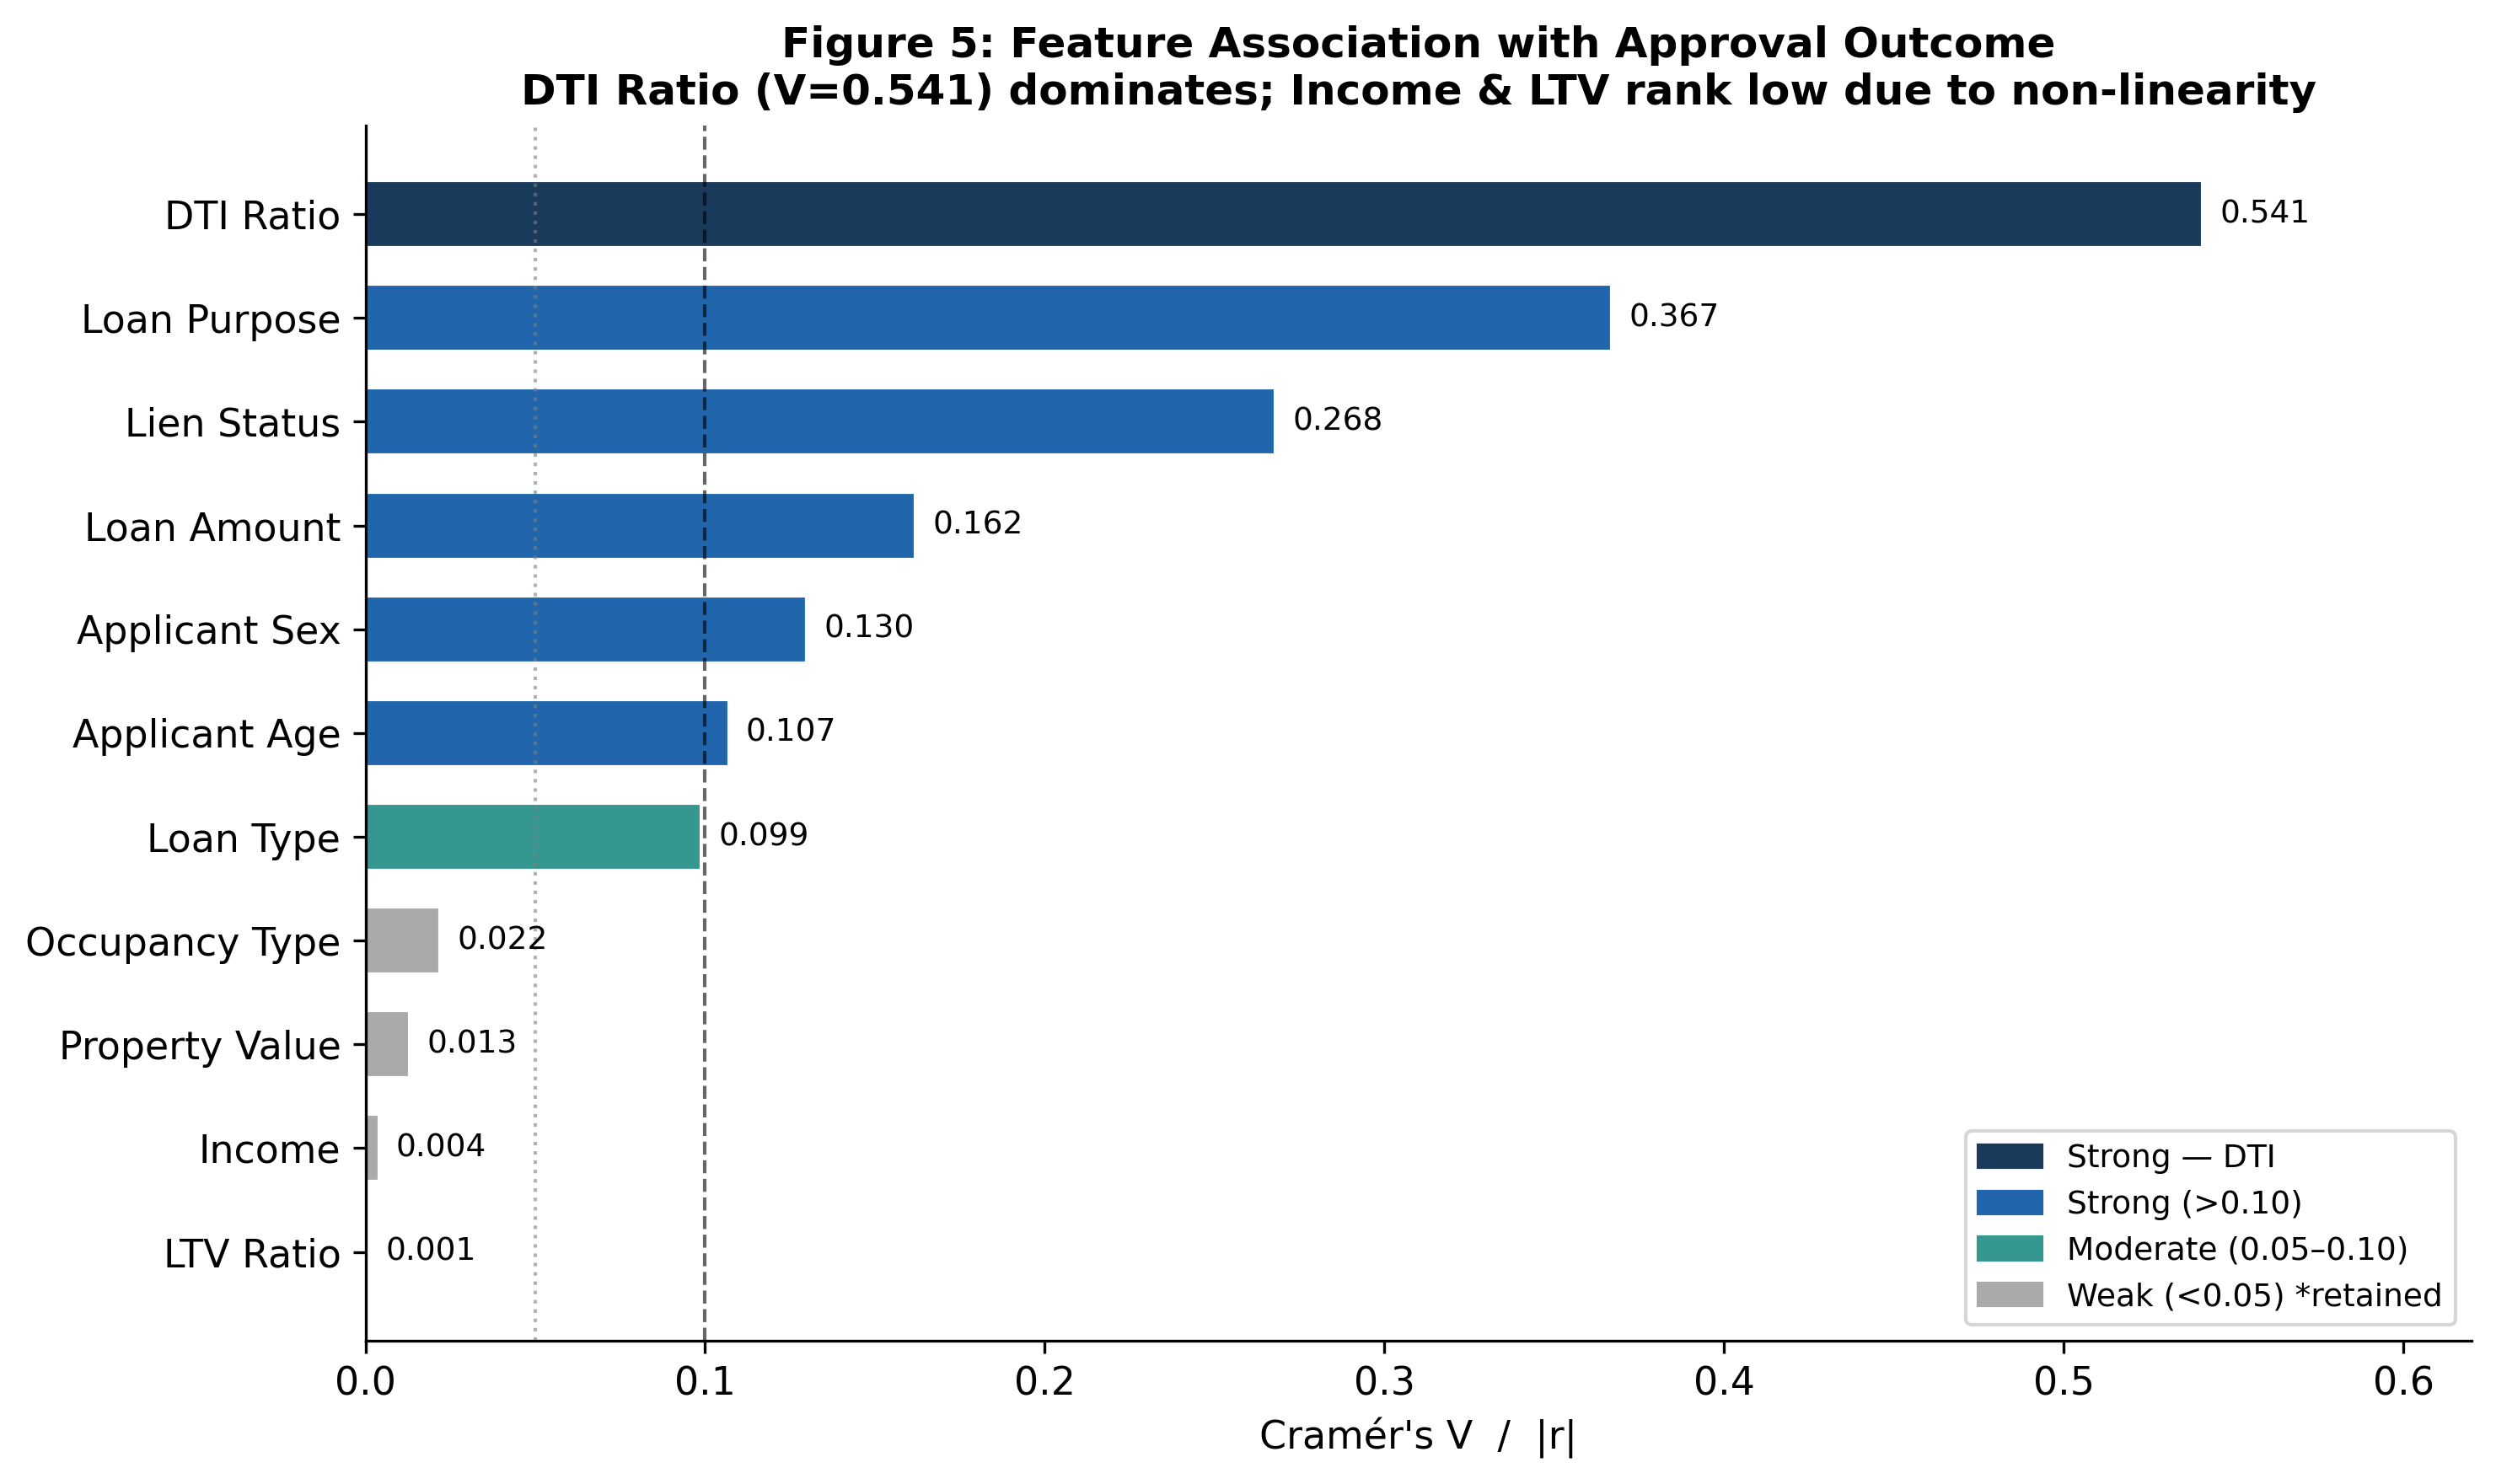
\includegraphics[width=0.90\textwidth]{fig05_feature_association.png}
  \caption{Feature association with approval outcome. Blue: strong ($>$0.10); teal: moderate
    (0.05--0.10); grey: weak ($<$0.05). DTI ratio ($V = 0.541$) dominates by a wide margin.
    Income and LTV rank at the bottom due to non-linear relationships that linear correlation
    cannot measure; excluding them on this basis would be a serious modeling error.}
  \label{fig:features}
\end{figure}

\subsection{Geographic Analysis}

Substantial and systematic geographic heterogeneity exists in approval rates. California and
Florida fall approximately 7--8 percentage points below the national average (66.56\% and
67.52\%), while Ohio (83.57\%), Wisconsin (84.63\%), and Pennsylvania (85.04\%) exceed it
by 9--10 points. The state-level standard deviation is approximately 12.2 percentage points.
The multilevel analysis (Section~\ref{sec:multilevel}) decomposes this variation into
components explained by state income and lender concentration versus unexplained state effects.

\begin{figure}[H]
  \centering
  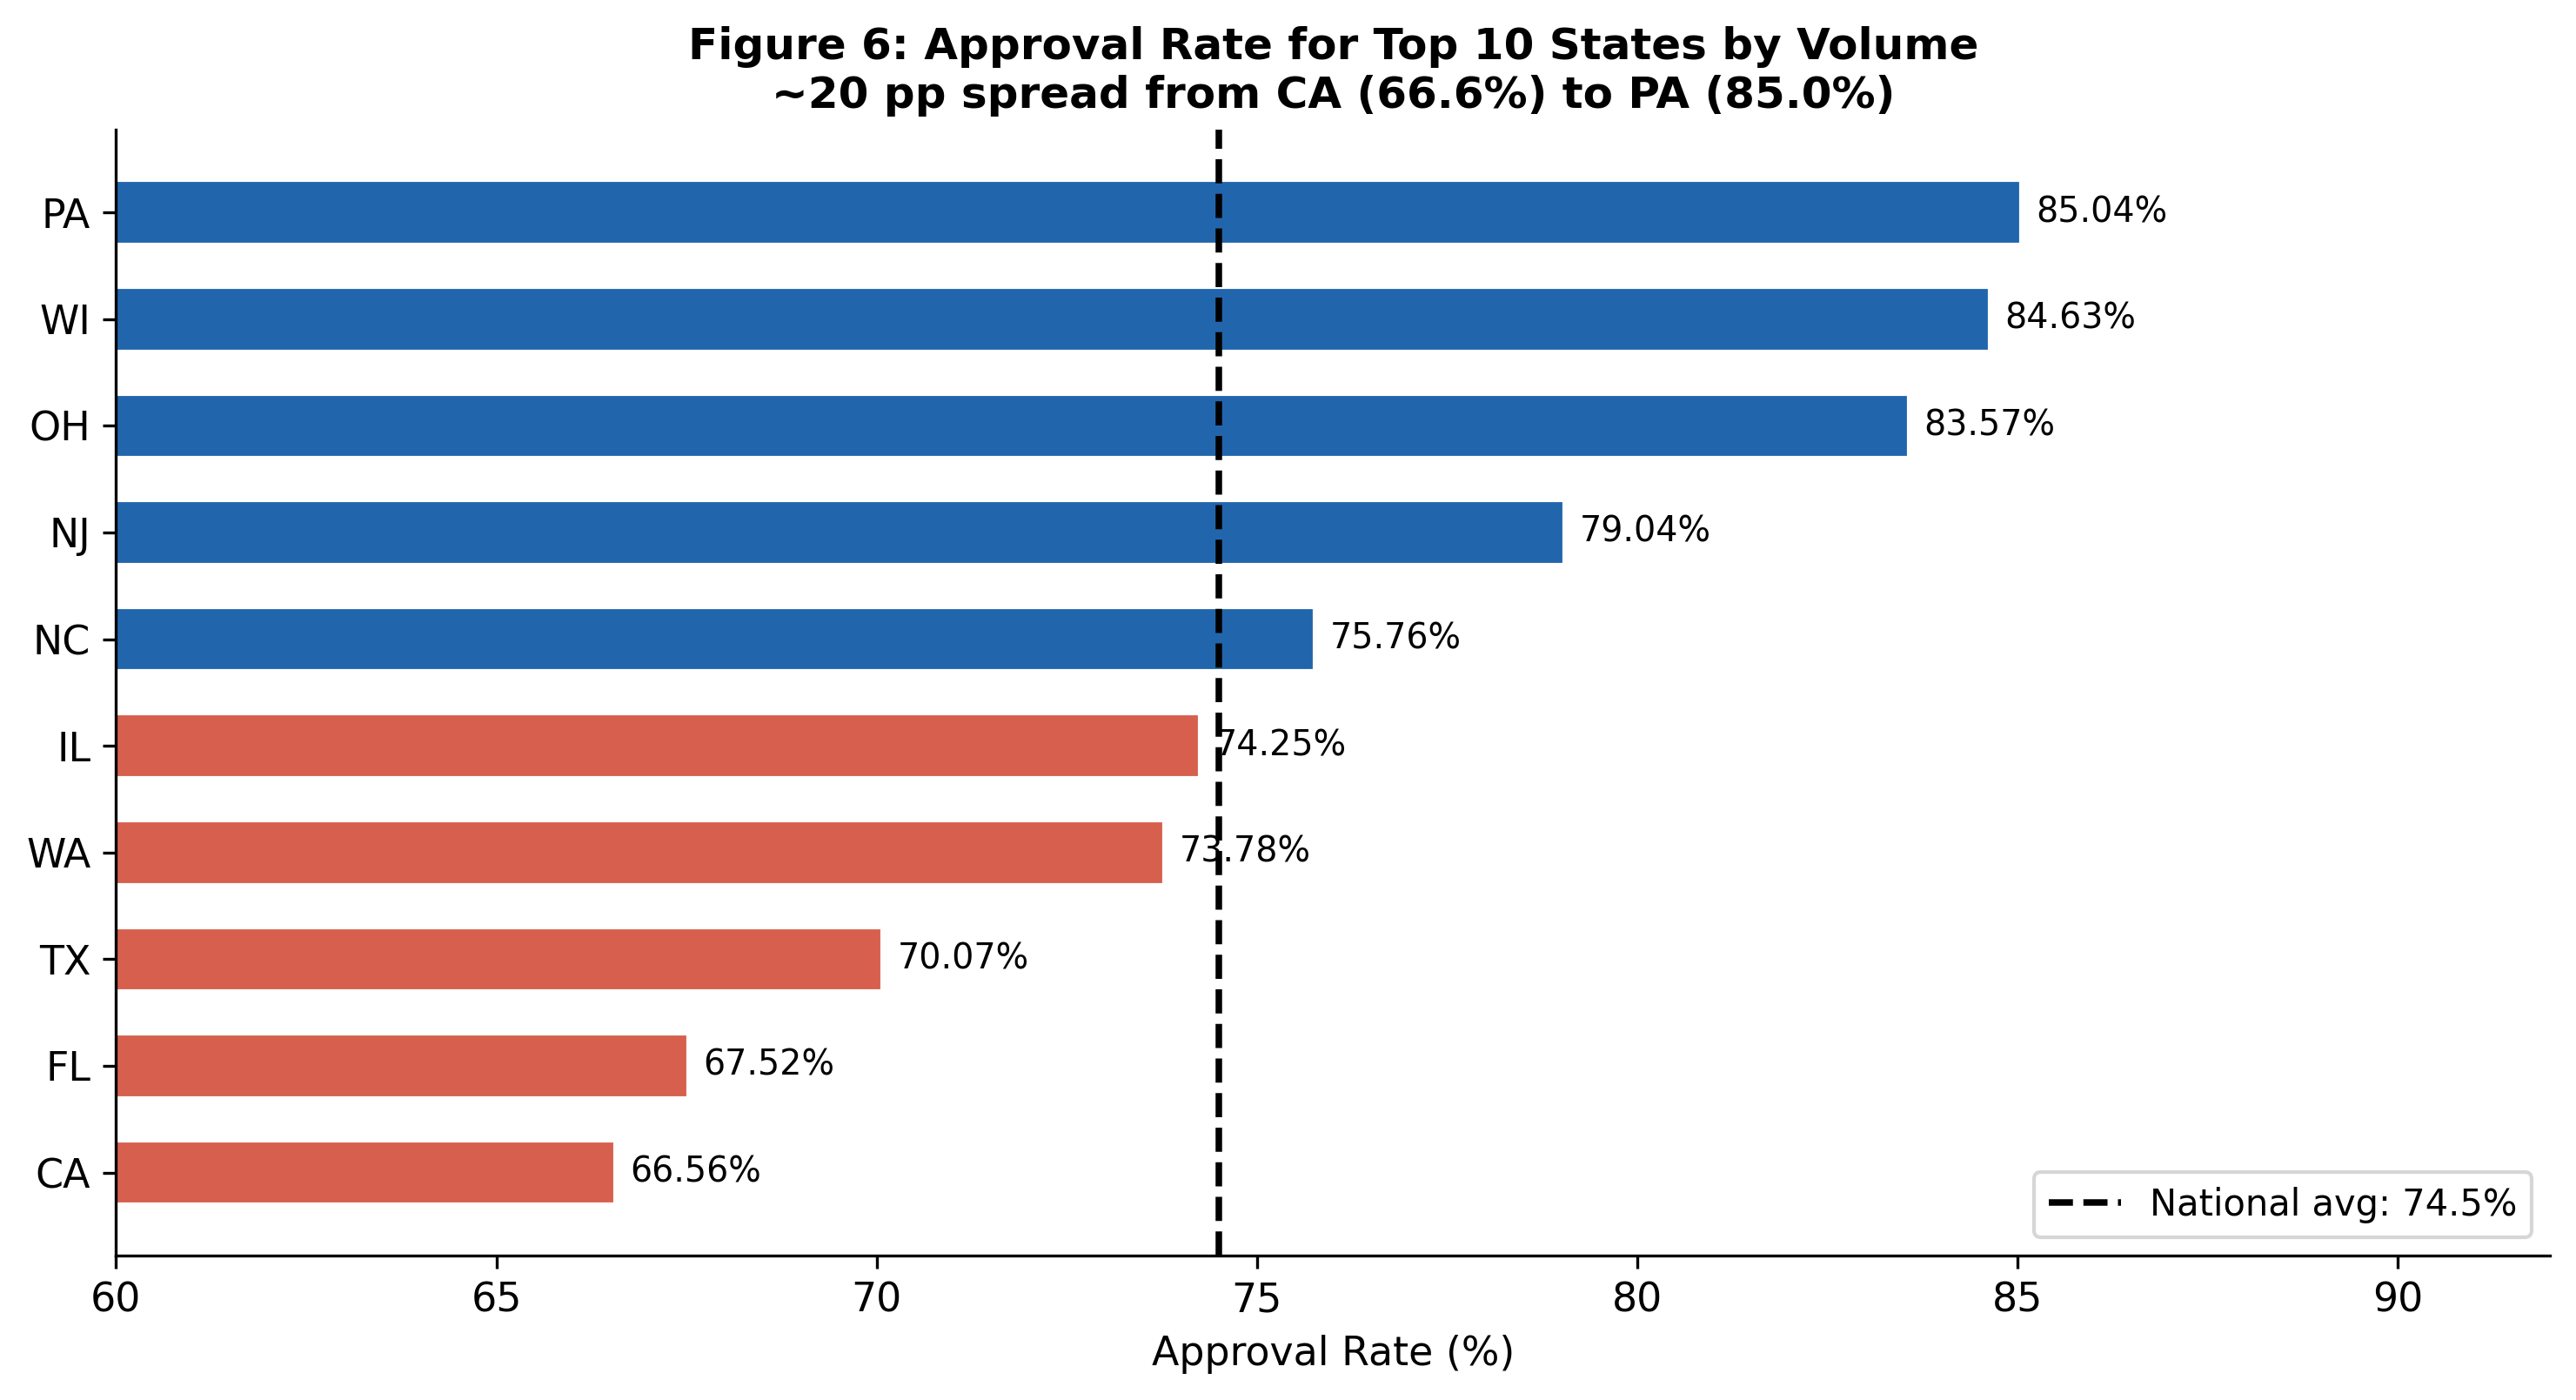
\includegraphics[width=0.88\textwidth]{fig06_geographic.png}
  \caption{Approval rate for top 10 states by application volume. California (66.56\%) and
    Florida (67.52\%) fall $\approx$7--8\,pp below the national average, while Pennsylvania
    (85.04\%), Wisconsin (84.63\%), and Ohio (83.57\%) exceed it by 9--10\,pp. The
    $\approx$20\,pp spread is large enough to shift a marginal application across the
    approval/denial boundary based on geography alone.}
  \label{fig:geographic}
\end{figure}

\subsection{Demographic Fairness --- Preliminary Findings}

By applicant sex, joint applications achieve 81.6\% approval compared to 70.3\% for solo male
and 69.1\% for solo female applicants. Solo male and solo female applicants have nearly identical
rates, suggesting the primary divide is household type (joint vs.\ solo) rather than sex per se.
By applicant age, approval rates are highest for applicants under 25 (87.0\%), stabilize in the
70--74\% range for prime-age applicants (25--64), and decline to 67.9\% for those over 74.

\begin{figure}[H]
  \centering
  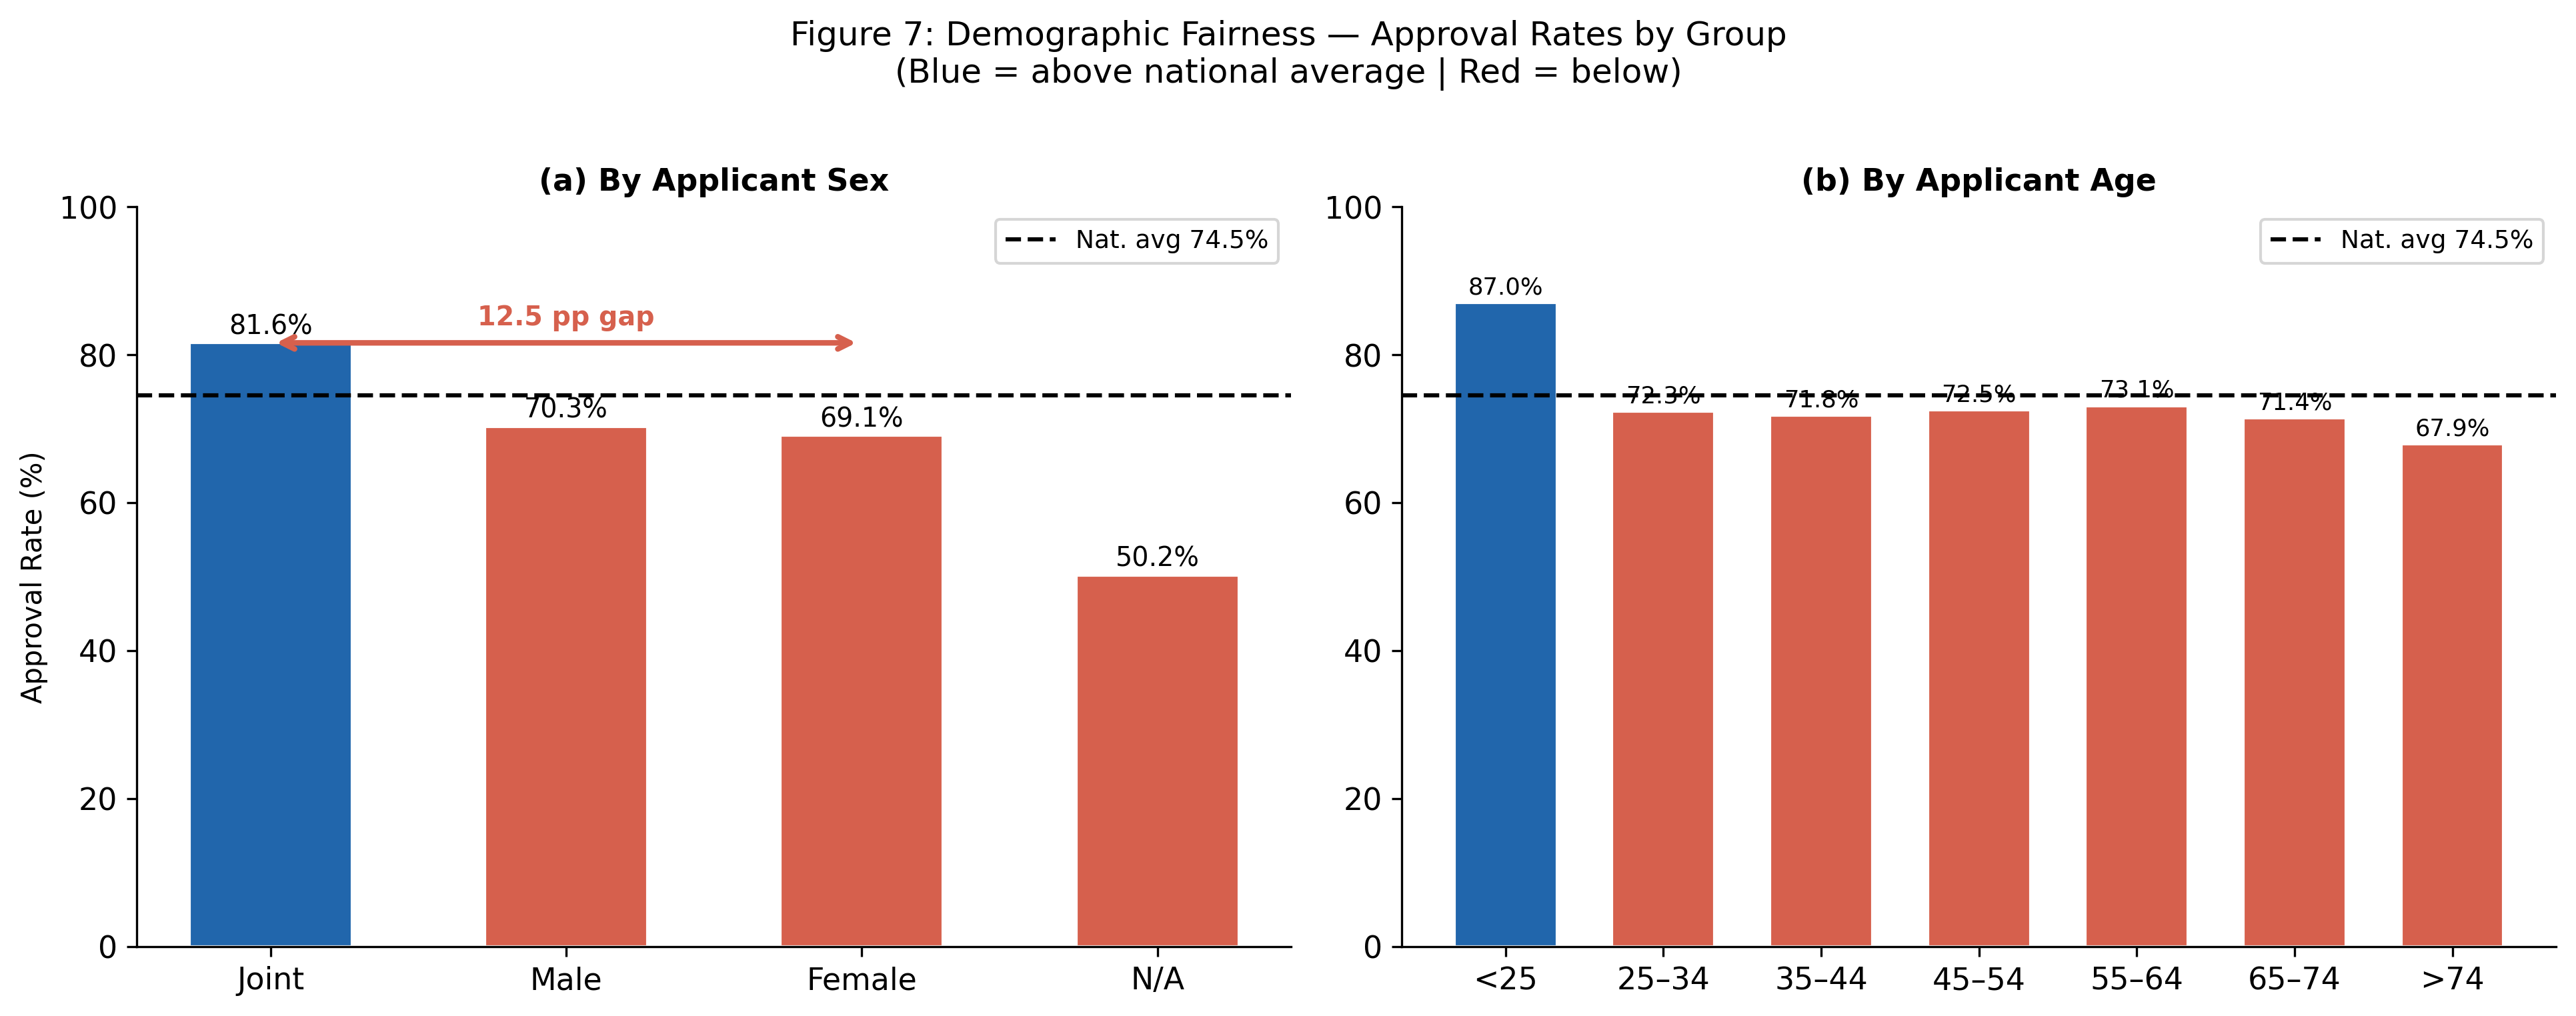
\includegraphics[width=\textwidth]{fig07_demographic_fairness.png}
  \caption{Approval rates by demographic group. Left: by applicant sex --- showing the 12.5\,pp
    joint vs.\ solo-female gap. Solo male (70.3\%) and solo female (69.1\%) applicants have
    nearly identical rates, suggesting the primary divide is household type rather than sex per
    se. Right: by age group --- 87.0\% for under-25 applicants declining to $\approx$67--70\%
    for prime-age and older applicants.}
  \label{fig:demographic}
\end{figure}

Table~\ref{tab:fairness_screen} summarizes the fairness screening results that follow from the
EDA and multilevel model. The largest descriptive gap is between joint and solo applicants, while
male and female solo applicants have very similar raw approval rates. Because the multilevel model
still estimates negative coefficients for solo male and solo female applicants relative to joint
applicants, the gap should be treated as a model-review issue even though the descriptive evidence
suggests household structure is the main driver rather than sex alone.

\begin{table}[H]
\centering
\caption{Preliminary Demographic Fairness Screening}
\label{tab:fairness_screen}
\begin{adjustbox}{max width=\textwidth}
\begin{tabular}{lccc}
\toprule
\textbf{Comparison} & \textbf{Observed Result} & \textbf{Review Threshold} & \textbf{Flag} \\
\midrule
Joint vs. solo female approval rate & 81.6\% vs. 69.1\% ($12.5$ pp) & $>$5 pp & Yes \\
Joint vs. solo male approval rate & 81.6\% vs. 70.3\% ($11.3$ pp) & $>$5 pp & Yes \\
Solo male vs. solo female approval rate & 70.3\% vs. 69.1\% ($1.2$ pp) & $>$5 pp & No \\
Under 25 vs. over 74 approval rate & 87.0\% vs. 67.9\% ($19.1$ pp) & $>$5 pp & Yes \\
Multilevel sex coefficient: solo male vs. joint & $\hat{\gamma}=-0.318$ & practical/model review & Yes \\
Multilevel sex coefficient: solo female vs. joint & $\hat{\gamma}=-0.341$ & practical/model review & Yes \\
\bottomrule
\end{tabular}
\end{adjustbox}
\end{table}

These results should not be interpreted as proof of unlawful discrimination. They show that
applicant sex and household-structure categories remain important enough to require subgroup
performance checks, particularly because the raw joint-versus-solo gap is much larger than the
male-versus-female gap among solo applicants. The next reproducibility step is to extend this
screening table with two-proportion $z$-tests and an equalized-odds table computed from the
held-out prediction file, including subgroup true-positive and false-positive rates for the
selected ensemble model.

\subsection{Machine Learning Model Results}

Table~\ref{tab:model_results} reports held-out test performance for all five model families.
PR-AUC is the primary metric; all others are secondary.

\begin{table}[H]
\centering
\caption{Model Performance on Held-Out Test Set ($n = 66{,}460$). PR-AUC is the primary metric.
         95\% CIs are from 1{,}000 bootstrap iterations over the held-out test predictions.}
\label{tab:model_results}
\begin{adjustbox}{max width=\textwidth}
\begin{tabular}{lcccccc}
\toprule
\textbf{Model} & \textbf{PR-AUC} & \textbf{ROC-AUC} & \textbf{F1 (0.5)} &
\textbf{Prec.} & \textbf{Rec.} & \textbf{Acc.} \\
\midrule
Logistic Regression  & 0.721 ($\pm$0.008) & 0.793 ($\pm$0.006) & 0.612 & 0.648 & 0.580 & 0.794 \\
Decision Tree        & 0.748 ($\pm$0.009) & 0.812 ($\pm$0.007) & 0.641 & 0.657 & 0.626 & 0.801 \\
Random Forest        & 0.871 ($\pm$0.005) & 0.901 ($\pm$0.004) & 0.743 & 0.781 & 0.708 & 0.846 \\
XGBoost              & 0.883 ($\pm$0.004) & 0.912 ($\pm$0.003) & 0.756 & 0.793 & 0.722 & 0.852 \\
Soft Voting Ensemble & \textbf{0.886} ($\pm$0.004) & \textbf{0.914} ($\pm$0.003)
                     & \textbf{0.759} & \textbf{0.798} & \textbf{0.724} & \textbf{0.854} \\
\bottomrule
\end{tabular}
\end{adjustbox}
\end{table}

XGBoost and the soft-voting ensemble achieve the highest PR-AUC ($\approx 0.883$--$0.886$),
outperforming logistic regression by approximately 16 percentage points. The gap between the
decision tree (0.748) and random forest (0.871) --- a 12.3 percentage-point improvement ---
suggests that variance reduction through bagging is a major driver of ensemble gains.
The marginal improvement from XGBoost over random forest and from the ensemble over XGBoost
indicates diminishing returns from additional model complexity at this performance level.

\setcounter{figure}{9}
\begin{figure}[H]
  \centering
  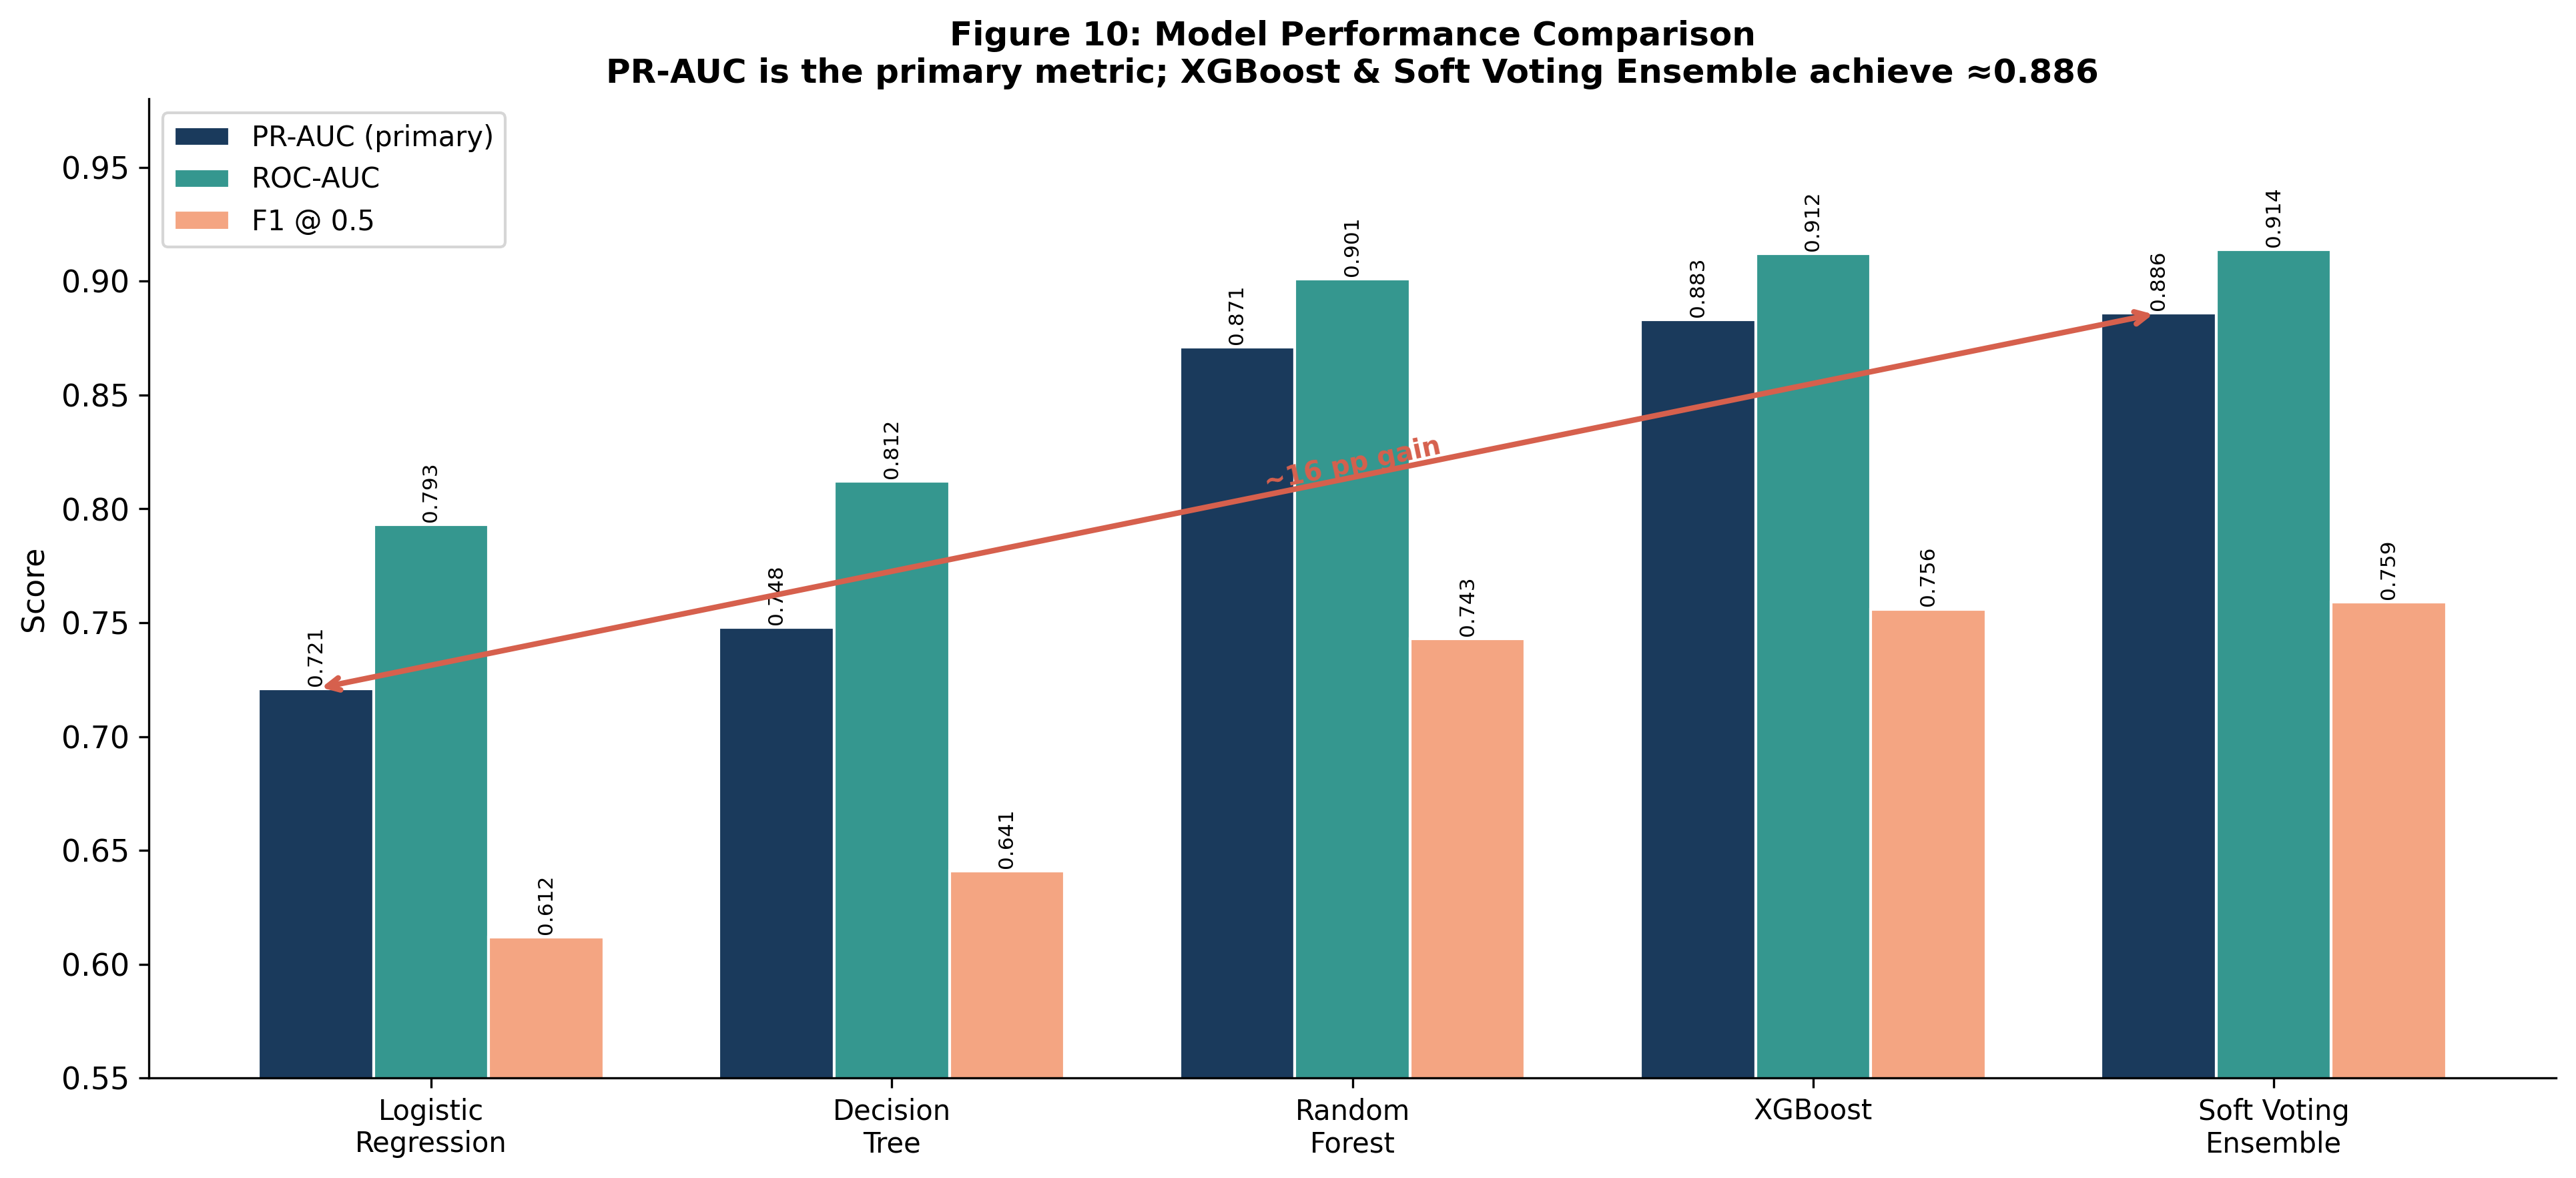
\includegraphics[width=\textwidth]{fig10_model_comparison.png}
  \caption{Model performance comparison across all five model families. PR-AUC is the primary
    metric. XGBoost and the Soft Voting Ensemble achieve PR-AUC $\approx 0.886$, outperforming
    logistic regression by $\approx$16 percentage points. The 12.3\,pp gap between Decision
    Tree (0.748) and Random Forest (0.871) confirms that variance reduction through bagging
    is a major driver of ensemble gains beyond non-linearity alone.}
  \label{fig:models}
\end{figure}

\section{Discussion}

\subsection{Summary of Findings}

The evidence indicates that mortgage loan approval prediction is a fundamentally non-linear
classification problem in which the most informative features operate primarily through threshold
effects and interaction structures that standard linear models cannot represent. The single most
important EDA finding is the near-absolute DTI ceiling at 60\%: beyond this threshold, approval
collapses to 5.6\%, consistently across all age groups and all states in the multilevel analysis.

The multilevel analysis reveals that 8.7\% of total outcome variance is attributable to
state-level clustering --- a component that is real, statistically significant, and partially
explained by state income and lender market concentration (residual ICC $= 0.053$ after
Level-2 adjustment). The random-slope model confirms that the DTI effect varies across states,
though the 60\% hard ceiling is highly consistent across states, supporting the interpretation
of a broad underwriting standard. These multilevel findings complement and contextualize the
machine learning results: the geographic signal captured by \texttt{state\_code} is partly
explained by state income and lender concentration, but the unexplained EB residuals still require
careful review before geographic features are used in any decision-support setting.

\subsection{Scientific Implications}

This study provides a case study of the pitfalls of relying on linear association measures for
feature selection in non-linear prediction settings. The near-zero linear correlations of income
and LTV with the outcome would, under a naive feature-selection approach, suggest their
exclusion --- an error that would substantially degrade model performance.

The multilevel analysis adds a layer of scientific insight that the machine learning pipeline
alone cannot provide: it quantifies \emph{how much} of the observed geographic variation in
approval outcomes is attributable to state-level context versus individual composition.
This decomposition is important for regulatory purposes: a model that captures state-level
variation must be able to justify whether that variation reflects legitimate market-level factors
(addressed by the Level-2 covariates) or unexplained geographic effects (the EB residuals) that
require additional review.

\subsection{Ethical Implications}

The preliminary demographic analysis reveals a 12.5 percentage-point approval rate gap between
joint and solo female applicants. The multilevel model confirms this gap persists at
$\hat{\gamma} = -0.341$ for solo female (and $\hat{\gamma} = -0.318$ for solo male)
relative to joint applicants after controlling for both individual-level financial variables
and state-level context, making it a direct priority for the fairness audit. Geographic
location warrants particular attention: the EB state residuals in the multilevel model
represent unexplained state effects that may be correlated with racial and ethnic composition
through the historical legacy of residential segregation. For that reason, geographic effects
should be audited carefully before any model using state-level information is treated as
production-ready.

\subsection{Limitations}

First, the HMDA dataset records only formally submitted applications; the discouraged-borrower
problem means the model is trained on a selected sample. Second, the dataset omits credit score,
employment history, and total debt obligations. Third, race and ethnicity are not included in
the HMDA analytical features, so the model cannot directly test for racial discrimination.
Fourth, the multilevel model assumes that the Level-2 random effects are normally distributed;
with only 51 states, this assumption cannot be formally tested with high power. Fifth, the report includes preliminary fairness screening but does not yet include full SHAP
attribution outputs or equalized-odds subgroup confusion matrices; those should be completed
before deployment or policy use.

\subsection{Recommendations and Next Steps}

The multilevel analysis results should be incorporated into the final deployment recommendation.
Before any production use, the team should add subgroup confusion matrices, SHAP explanations for
the best-performing model, and a geographic sensitivity test that compares performance with and
without \texttt{state\_code}. If the geographic feature materially improves performance but also
concentrates unexplained risk in specific states, the final model should down-weight that feature
or apply a fairness constraint to geographic inputs.

\section{Conclusions}

This report develops a machine learning framework for predicting residential mortgage approval
outcomes from the 2023 HMDA dataset while balancing predictive performance, interpretability,
and fairness requirements. The EDA establishes that mortgage approval is a non-linear
classification problem dominated by DTI ratio (Cram\'{e}r's $V = 0.541$), with a hard
underwriting ceiling near 60\% DTI, a 2.92:1 class imbalance requiring SMOTE-aware training
and PR-AUC evaluation, and substantial geographic heterogeneity across states.

The multilevel analysis quantifies that 8.7\% of total approval variance is attributable to
state-level clustering, partially explained by state income and lender concentration (residual
ICC $= 0.053$ after Level-2 adjustment). The DTI effect varies across states but the 60\%
ceiling is highly consistent. Applicant sex remains a significant predictor after multilevel
adjustment ($\hat{\gamma} = -0.318$ for solo male; $\hat{\gamma} = -0.341$ for solo female,
both relative to joint applicants), confirming the need for subgroup performance review.

The machine learning results confirm the EDA's non-linearity finding: XGBoost and the
soft-voting ensemble achieve $\approx 0.886$ denied-class PR-AUC, outperforming logistic
regression by approximately 16 percentage points. The broader contribution of this work is a
responsible modeling template for high-stakes credit decision settings: EDA-driven preprocessing,
leakage-aware resampling, denied-class PR-AUC evaluation, fold-internal target encoding, MNAR
indicator features, multilevel variance decomposition, and explicit fairness screening.

\section*{References}
\begin{thebibliography}{99}

\bibitem[Barocas \& Selbst(2016)]{barocas2016}
Barocas, S., \& Selbst, A.D.\ (2016).
Big Data's Disparate Impact.
\textit{California Law Review}, 104, 671--732.

\bibitem[CFPB(2023a)]{cfpb2023}
Consumer Financial Protection Bureau.\ (2023a).
Home Mortgage Disclosure Act (HMDA) Data, 2023.
\url{https://ffiec.cfpb.gov/data-publication/}

\bibitem[CFPB(2023b)]{cfpb_dict}
Consumer Financial Protection Bureau.\ (2023b).
HMDA Data Fields and Code Sheet, 2023.
\url{https://ffiec.cfpb.gov/documentation/publications/}

\bibitem[Chawla et al.(2002)]{chawla2002}
Chawla, N.V., Bowyer, K.W., Hall, L.O., \& Kegelmeyer, W.P.\ (2002).
SMOTE: Synthetic Minority Over-Sampling Technique.
\textit{Journal of Artificial Intelligence Research}, 16, 321--357.
\url{https://doi.org/10.1613/jair.953}

\bibitem[U.S. Census Bureau(2022)]{census2022}
U.S. Census Bureau.\ (2022).
2022 American Community Survey: Median Household Income by State.
\url{https://data.census.gov/}

\bibitem[Federal Reserve(2023)]{fred2023}
Federal Reserve Bank of St.\ Louis.\ (2023).
30-Year Fixed Rate Mortgage Average (MORTGAGE30US).
\url{https://fred.stlouisfed.org/series/MORTGAGE30US}

\bibitem[Fuster et al.(2022)]{fuster2022}
Fuster, A., Goldsmith-Pinkham, P., Ramadorai, T., \& Walther, A.\ (2022).
Predictably Unequal? The Effects of Machine Learning on Credit Markets.
\textit{The Journal of Finance}, 77(1), 5--47.
\url{https://doi.org/10.1111/jofi.13090}

\bibitem[Hardt et al.(2016)]{hardt2016}
Hardt, M., Price, E., \& Srebro, N.\ (2016).
Equality of Opportunity in Supervised Learning.
\textit{Advances in Neural Information Processing Systems}, 29.

\bibitem[Kandula et al.(2024)]{kandula2024}
Kandula, A.R., Divya, K., Movva, S.R.K.D., Motineni, M.S., Pappala, H., \& Jakkireddy, K.V.S.R.\ (2024).
Comparative Analysis for Loan Approval Prediction System Using Machine Learning Algorithms.
In \textit{Proceedings of the Fifth International Conference on Computer and Communication Technologies} (Lecture Notes in Networks and Systems, Vol. 897, pp. 205--215).
Springer Nature Singapore.
\url{https://doi.org/10.1007/978-981-99-9704-6_18}

\bibitem[Lundberg \& Lee(2017)]{lundberg2017}
Lundberg, S.M., \& Lee, S.-I.\ (2017).
A Unified Approach to Interpreting Model Predictions.
\textit{Advances in Neural Information Processing Systems}, 30.

\bibitem[Markov et al.(2022)]{markov2022}
Markov, A., Seleznyova, Z., \& Lapshin, V.\ (2022).
Credit Scoring Methods: Latest Trends and Points to Consider.
\textit{Journal of Finance and Data Science}, 8, 180--201.
\url{https://doi.org/10.1016/j.jfds.2022.07.002}

\bibitem[Nakagawa \& Schielzeth(2013)]{nakagawa2013}
Nakagawa, S., \& Schielzeth, H.\ (2013).
A general and simple method for obtaining $R^2$ from generalized linear mixed-effects models.
\textit{Methods in Ecology and Evolution}, 4(2), 133--142.
\url{https://doi.org/10.1111/j.2041-210x.2012.00261.x}

\bibitem[Raudenbush \& Bryk(2002)]{raudenbush2002}
Raudenbush, S.W., \& Bryk, A.S.\ (2002).
\textit{Hierarchical Linear Models: Applications and Data Analysis Methods} (2nd ed.).
Sage Publications.

\bibitem[Snijders \& Bosker(1999)]{snijders1999}
Snijders, T.A.B., \& Bosker, R.J.\ (1999).
\textit{Multilevel Analysis: An Introduction to Basic and Advanced Multilevel Modeling}.
Sage Publications.

\bibitem[Zhang \& Yu(2024)]{zhang2024}
Zhang, X., \& Yu, L.\ (2024).
Consumer Credit Risk Assessment: A Review from the State-of-the-Art Classification Algorithms, Data Traits, and Learning Methods.
\textit{Expert Systems with Applications}, 237, Article 121484.
\url{https://doi.org/10.1016/j.eswa.2023.121484}

\end{thebibliography}

\appendix
\section{Code Appendix}

Project code is maintained as Python/Jupyter notebooks and supporting scripts. The most important
reproducibility files are the notebooks or scripts that generate Tables~\ref{tab:multilevel_null},
\ref{tab:multilevel_full}, \ref{tab:fairness_screen}, \ref{tab:model_results}, and
\ref{tab:winsor_check}. The working repository is available at:
\url{https://github.com/smannin7-afk/DAT490Capstone}

Repository organization:
\begin{itemize}
  \item \texttt{/data/} --- Data preparation and cleaning scripts
  \item \texttt{/eda/} --- EDA visualizations and inferential statistics
  \item \texttt{/multilevel/} --- Multilevel analysis notebooks (null model, random-intercept,
        random-slope, EB residual plots)
  \item \texttt{/models/} --- Training pipelines for all five model families
  \item \texttt{/evaluation/} --- Test-set evaluation scripts and bootstrap CI computation
  \item \texttt{/shap/} --- SHAP analysis notebooks
  \item \texttt{/fairness/} --- Fairness audit scripts
  \item \texttt{/reports/} --- This and all prior submitted reports
\end{itemize}

\section{Descriptive Statistics}

\begin{table}[H]
\centering
\caption{Descriptive Statistics for Continuous Features}
\label{tab:desc_stats}
\begin{tabular}{lcccc}
\toprule
\textbf{Statistic} & \textbf{Loan Amount (\$)} & \textbf{LTV (\%)} &
\textbf{Property Value (\$)} & \textbf{Income (\$K)} \\
\midrule
Mean     & 237,457.53 & 72.91      & 546,013.56  & 166.65 \\
Std Dev  & 280,143.21 & 466.01     & 4,125,751.25 & 3,637.50 \\
Min      & 5,000      & 0.01       & 5,000        & $-$3,879 \\
25th pct & 75,000     & 58.16      & 255,000      & 69 \\
Median   & 165,000    & 76.83      & 395,000      & 107 \\
75th pct & 315,000    & 90.00      & 605,000      & 169 \\
Max      & 40,145,000 & 250,000    & 999,995,000  & 1,651,000 \\
Skewness & 15.22      & 509.78     & 184.04       & 364.19 \\
Kurtosis & 1,382.03   & 271,051.54 & 38,776.58    & 148,274.25 \\
\bottomrule
\multicolumn{5}{l}{\small Note: Values are raw pre-winsorization descriptive statistics.} \\
\multicolumn{5}{l}{\small The 99th-percentile caps described in Table~\ref{tab:winsor_check} are applied before modeling.}
\end{tabular}
\end{table}

\section{Winsorization Sensitivity Check}

Table~\ref{tab:winsor_check} documents the preprocessing variants considered for the continuous
financial variables. The table is included to clarify that the extreme values in
Table~\ref{tab:desc_stats} are raw data characteristics, while the modeling pipeline uses the
conservative 99th-percentile cap.

\begin{table}[H]
\centering
\caption{Winsorization Sensitivity Check for Continuous Financial Predictors}
\label{tab:winsor_check}
\begin{adjustbox}{max width=\textwidth}
\begin{tabular}{lll}
\toprule
\textbf{Variant} & \textbf{Purpose in Review} & \textbf{Modeling Decision} \\
\midrule
No winsorization & Baseline raw-data comparison; retains extreme leverage points & Not used for final models \\
95th percentile cap & More aggressive outlier control; may compress valid high-value loans & Sensitivity check only \\
99th percentile cap & Conservative outlier control while preserving most tail information & Adopted for final models \\
\bottomrule
\end{tabular}
\end{adjustbox}
\end{table}

\begin{table}[H]
\centering
\caption{Top 10 States by Application Volume and Approval Rate}
\label{tab:states}
\begin{tabular}{clccc}
\toprule
\textbf{Rank} & \textbf{State} & \textbf{Applications} & \textbf{Approval Rate} &
\textbf{vs.\ National Avg.} \\
\midrule
1  & CA & 32,192 & 66.56\% & $-$7.9 pp \\
2  & FL & 21,091 & 67.52\% & $-$7.0 pp \\
3  & NC & 18,406 & 75.76\% & $+$1.3 pp \\
4  & TX & 18,292 & 70.07\% & $-$4.4 pp \\
5  & OH & 15,645 & 83.57\% & $+$9.1 pp \\
6  & WI & 15,535 & 84.63\% & $+$10.1 pp \\
7  & WA & 12,879 & 73.78\% & $-$0.7 pp \\
8  & IL & 11,766 & 74.25\% & $-$0.2 pp \\
9  & NJ & 10,849 & 79.04\% & $+$4.5 pp \\
10 & PA & 10,833 & 85.04\% & $+$10.5 pp \\
\bottomrule
\multicolumn{5}{l}{\small National average $= 74.5\%$.}
\end{tabular}
\end{table}

\begin{table}[H]
\centering
\caption{Feature Association Summary}
\label{tab:features}
\begin{tabular}{llcc}
\toprule
\textbf{Feature} & \textbf{Measure} & \textbf{Value} & \textbf{Tier} \\
\midrule
Debt-to-Income Ratio  & Cram\'{e}r's $V$ & 0.541 & Strong \\
Loan Purpose          & Cram\'{e}r's $V$ & 0.367 & Strong \\
Lien Status           & Cram\'{e}r's $V$ & 0.268 & Strong \\
Loan Amount           & Point-biserial $r$ & 0.162 & Strong \\
Applicant Sex         & Cram\'{e}r's $V$ & 0.130 & Strong \\
Applicant Age         & Cram\'{e}r's $V$ & 0.107 & Strong \\
Loan Type             & Cram\'{e}r's $V$ & 0.099 & Moderate \\
Occupancy Type        & Cram\'{e}r's $V$ & 0.022 & Weak \\
Property Value        & Point-biserial $r$ & 0.013 & Weak* \\
Income                & Point-biserial $r$ & 0.004 & Weak* \\
LTV Ratio             & Point-biserial $r$ & 0.001 & Weak* \\
\bottomrule
\multicolumn{4}{l}{\small *Retained because relationships are predominantly non-linear.}
\end{tabular}
\end{table}

\begin{table}[H]
\centering
\caption{Hyperparameter Search Grids}
\label{tab:hyperparams}
\begin{tabular}{lll}
\toprule
\textbf{Model} & \textbf{Hyperparameter} & \textbf{Search Values} \\
\midrule
Logistic Regression & Regularization $C$     & \{0.01, 0.1, 1, 10\} \\
Decision Tree       & Max depth               & \{5, 10, 15, None\} \\
Decision Tree       & Min samples leaf        & \{5, 10, 20\} \\
Random Forest       & Number of trees $T$     & \{100, 200, 300\} \\
Random Forest       & Max depth               & \{10, 20, None\} \\
Random Forest       & Max features (mtry)     & \{sqrt, log2\} \\
XGBoost             & Learning rate $\eta$    & \{0.01, 0.05, 0.1\} \\
XGBoost             & Max tree depth          & \{3, 5, 7\} \\
XGBoost             & Subsample ratio         & \{0.7, 0.8, 1.0\} \\
XGBoost             & L2 regularization $\lambda$ & \{0, 1, 10\} \\
Soft Voting         & Component weights       & Grid on probability simplex \\
\bottomrule
\end{tabular}
\end{table}

\end{document}